\documentclass[main.tex,fontsize=12pt,paper=a4,paper=landscape,DIV=calc,]{scrartcl}
% Document
\usepackage[T1]{fontenc}
\usepackage[utf8]{inputenc}
\usepackage[dvipsnames]{xcolor}
\usepackage[nswissgerman,english]{babel} 
\usepackage{hyperref}
\renewcommand{\familydefault}{\sfdefault}

% Format
\usepackage[top=5mm,bottom=5mm,left=5mm,right=5mm]{geometry}
%\setlength{\headheight}{\baselineskip}
%\setlength{\headsep}{0mm}

%\usepackage{scrlayer-scrpage}
%\clearpairofpagestyles
%\chead{{\bfseries\TITLE, \AUTHOR, \pagename~\thepage}}

%\addtokomafont{pagehead}{\upshape}

\usepackage{multicol}
\setlength{\columnsep}{2mm}
\setlength{\columnseprule}{0.1pt}

% Math
\usepackage{amsmath}
\usepackage{amssymb}
\usepackage{amsfonts}

% Code
\usepackage{fancyvrb, etoolbox, listings, xcolor}
%\usemintedstyle{bw}

%\newminted[shell]{bash}{
%fontsize=\footnotesize,
%fontfamily=tt,
%breaklines=true,
%frame=single,
%framerule=0.1pt,
%framesep=2mm,
%tabsize=2
%}
%\newminted{css}{
%breaklines=true,
%tabsize=4,
%autogobble=true,
%escapeinside=||,
%stripall=true,
%stripnl=true,
%}

    \definecolor{lightgray}{rgb}{0.95, 0.95, 0.95}
    \definecolor{darkgray}{rgb}{0.4, 0.4, 0.4}
    \definecolor{purple}{rgb}{0.65, 0.12, 0.82}
    \definecolor{ocherCode}{rgb}{1, 0.5, 0} % #FF7F00 -> rgb(239, 169, 0)
    \definecolor{blueCode}{rgb}{0, 0, 0.93} % #0000EE -> rgb(0, 0, 238)
    \definecolor{greenCode}{rgb}{0, 0.6, 0} % #009900 -> rgb(0, 153, 0)
    \definecolor{teal}{rgb}{0.0, 0.5, 0.5}

\lstdefinestyle{code}{
    identifierstyle=\color{black},
    keywordstyle=\color{blue}\bfseries\small,
    ndkeywordstyle=\color{greenCode}\bfseries\small,
    stringstyle=\color{ocherCode}\ttfamily\small,
    commentstyle=\color{teal}\ttfamily\textit\small,
    basicstyle=\ttfamily\small,
    breakatwhitespace=false,         
    breaklines=true,                 
    captionpos=b,                    
    keepspaces=true,                 
    showspaces=false,                
    showstringspaces=false,
    showtabs=false,                  
    tabsize=2,
    belowskip=-5pt
}



% Images
\usepackage{graphicx}
\newcommand{\pic}{\includegraphics[scale=0.3]}
\graphicspath{{Screenshots/}{../Screenshots}}
\makeatletter
\def\pictext#1#2{%
    \@ifnextchar[{%
    \pictext@iiiii{#1}{#2}%
    }{%
      \pictext@iiiii{#1}{#2}[0.5,0.4,0.3]% Default is 5
    }%
}
\def\pictext@iiiii#1#2[#3,#4,#5]{\begin{minipage}{#3\textwidth}\includegraphics[scale=#4]{#1}\end{minipage}\begin{minipage}{#5\textwidth}#2\end{minipage}}
\def\minipg#1#2{%
    \@ifnextchar[{%
    \minipg@iiii{#1}{#2}%
    }{%
      \minipg@iiii{#1}{#2}[0.3,0.6]% Default is 5
    }%
}
\def\minipg@iiii#1#2[#3,#4]{\vspace{0.8mm}\begin{minipage}{#3\textwidth}#1\end{minipage}\begin{minipage}{#4\textwidth}#2\end{minipage}{\vspace{0.8mm}}}
\makeatother

%\newenvironment{minty}[2]% environment name
%{% begin code
%  \begin{minipage}{#1}
%  \begin{minted}{#2}
%}%
%{% end code
%  \end{minted}
%  \end{minipage}
%  \end{minty}\ignorespacesafterend
%} 

% Smaller Lists
\usepackage{enumitem}
\setlist[itemize,enumerate]{leftmargin=3mm, labelindent=0mm, labelwidth=1mm, labelsep=1mm, nosep}
\setlist[description]{leftmargin=0mm, nosep}
\setlength{\parindent}{0cm}

% Smaller Titles
\usepackage[explicit]{titlesec}

%% Color Boxes
\newcommand{\sectioncolor}[1]{\colorbox{black!60}{\parbox{0.97\linewidth}{\color{white}#1}}}
\newcommand{\subsectioncolor}[1]{\colorbox{black!50}{\parbox{0.97\linewidth}{\color{white}#1}}}
\newcommand{\subsubsectioncolor}[1]{\colorbox{black!40}{\parbox{0.97\linewidth}{\color{white}#1}}}
\newcommand{\paragraphcolor}[1]{\colorbox{black!30}{\parbox{0.97\linewidth}{\color{white}#1}}}
\newcommand{\subparagraphcolor}[1]{\colorbox{black!20}{\parbox{0.97\linewidth}{\color{white}#1}}}

%% Title Format
\titleformat{\section}{\vspace{0.3mm}\bfseries}{}{0mm}{\sectioncolor{\thesection~#1}}[{\vspace{0.3mm}}]
\titleformat{\subsection}{\vspace{0.3mm}\bfseries}{}{0mm}{\subsectioncolor{\thesubsection~#1}}[{\vspace{0.3mm}}]
\titleformat{\subsubsection}{\vspace{0.3mm}\bfseries}{}{0mm}{\subsubsectioncolor{\thesubsubsection~#1}}[{\vspace{0.3mm}}]
\titleformat{\paragraph}{\vspace{0.3mm}\bfseries}{}{0mm}{\paragraphcolor{\theparagraph~#1}}[{\vspace{0.3mm}}]
\titleformat{\subparagraph}{\vspace{0.3mm}\bfseries}{}{0mm}{\subparagraphcolor{\thesubparagraph~#1}}[{\vspace{0.3mm}}]

%% Title Spacing
\titlespacing{\section}{0mm}{0mm}{0mm}
\titlespacing{\subsection}{0mm}{0mm}{0mm}
\titlespacing{\subsubsection}{0mm}{0mm}{0mm}
\titlespacing{\paragraph}{0mm}{0mm}{0mm}
\titlespacing{\subparagraph}{0mm}{0mm}{0mm}

%% format cells
\usepackage[document]{ragged2e}
\usepackage{array, makecell}
\renewcommand{\arraystretch}{2}
\newcommand{\mc}{\makecell[{{m{1\linewidth}}}]}




\begin{document}

\tableofcontents
\pagebreak 

\begin{multicols*}{2}
\section{The magical Triangle}
\textcolor{purple}{Cost - Scope - Time}
The simple problem that these all conflict with each other.\newline
A bigger scope requires more development salary and more time.\newline
While less time needs more developers or a smaller scope.

\section{Circle of Quality according to Deming}
This is a plan to fix problems that you find in your project.\newline
\begin{itemize}
\item \textcolor{purple}{Plan}\newline
  Create a plan to fix the issue:\newline
  \textcolor{orange}{Think \textbf{SMART}}\newline
  \begin{itemize}
  \item \textcolor{black}{Specifc}
  \item \textcolor{black}{Measured}
  \item \textcolor{black}{Accepted}
  \item \textcolor{black}{Realistic}
  \item \textcolor{black}{Terminated}
  \end{itemize} 
\item \textcolor{purple}{Do}\newline 
  Test the plan with a small sample:\newline
  \textcolor{orange}{OTOBOS}\newline
  \begin{itemize}
  \item \textcolor{black}{OT: On Time}
  \item \textcolor{black}{OB: On Budget}
  \item \textcolor{black}{OS: On Scope}
  \end{itemize} 
\item \textcolor{purple}{Check}\newline
  Check the results of that sample:\newline
  \textcolor{orange}{Mind the gap}\newline
  Find errors fast and correct them before they get expensive down the line!
\item \textcolor{purple}{Act}\newline
  Implement this for the entire company/project
\end{itemize} 

\section{Project Controlling}
\subsection{Project Manager}
This person specifies how, what and when, however, this person should not be the same person that will evaluate whether or not the project is going according to plan! \newline

\subsection{Project Controller}
This person is the one who will check whether or not the measures and structures that the project manager has implemented work as intended, and if they even make sense.\newline
The project controller is assigned by the project manager and works according to what the project manager has laid out.\newline
\textcolor{teal}{Note this sounds like some waterfall crap}\newline

\subsection{Traffic Light principle}
\minipg{
The traffic light specifies whether there are any deviations in the project from what you had planned.\newline
Note that the amount of deviation needed for red or yellow depends on the project (yellow usually 0-5\% and red > 5\%).\newline
\textbf{Yellow says that you need to take a close look at the issue, and red means escalation.}\newline
\textcolor{purple}{Note that yellow or red will always take precedence, meaning that if one aspect of the project is red, then the entire project is considered red.}\newline
}{
  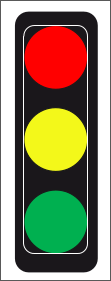
\includegraphics[scale=0.4]{2023_01_09_02_24_00.png}
}[0.4,0.25]

\subsection{Earned-Value-Analysis}
\begin{itemize}
  \item \textcolor{purple}{Planned Cost(PV)}
\item \textcolor{purple}{Actual Cost(AC)}
\item \textcolor{purple}{Earned Value(EV)}
\item \textcolor{purple}{Cost Variance(CV) = EV - AC}\newline
\item \textcolor{purple}{Cost Performance Index(CPI) = \(\dfrac{\text{EV}}{\text{AC}}\)}
\end{itemize} 
\textcolor{teal}{The goal is to have the CPI > 1, obviously.}

\subsection{Earned-Value Evaluation}
\begin{itemize}
\item \textcolor{orange}{Strict variant}\newline
  This variant simply states that the EV is 0 until we actually have the product/software.\newline
  In other words 0 until completion.
\item \textcolor{orange}{Variant current scope}\newline
  This evaluates the current EV with the current cost as specified above
\item \textcolor{orange}{Variant Rest}\newline
  This take the current time and looks ahead at what we still need to do until we have the complete product.\newline
  Ex: If we have planned 300h with 100Fr/h, and we notice after 150h spent that we have 200h of work left instead of 150, then we need to calculate the rest for the 200h.\newline
\end{itemize} 
\, \newline
\large \textcolor{purple}{\(\text{EV} = \dfrac{\text{PC}}{\text{AC + REST}} * \text{AC}\)}\newline
\normalsize \, \newline
\(\text{EV} = \dfrac{300\text{h} * 100\text{Fr}}{150\text{h} * 100\text{Fr.} + 200\text{h} * 100\text{Fr.}} * 150\text{h} * 100\text{Fr.} \)

\subsection{Milestones} 
Milestones are measured in intervals to see if they are completed at that time.\newline
If too many milestones can't hit their timeframe according to analysis, then the project needs to be canceled.

\section{Requirement Engineering} 
Here we define the user stories with UML diagrams etc, in order to define what exactly we need to do.\newline
This is necessary as customers have often not an exact idea about the program they want/need, as they are not used to deal with this subject.\newline
\textcolor{purple}{Note the verbs used in the userstories or requirements(depends on agile or waterfall) -> must vs should\newline
The should is an optional thing that can be left out if not possible or no time is left for this, while must is a base requirement.} 

\section{Models: Agile vs Classic}
\subsection{Waterfall, a classic approach}
\begin{itemize}
\item \textcolor{black}{Each Milestone is done in order}
\item \textcolor{black}{Each Milestone is finished completely until next milestone is started}\newline
  There are no parallel milestones!
\item \textcolor{black}{Clear and fixed structures}
\item \textcolor{black}{Project status is always obvious and apparent}
\end{itemize} 
\textcolor{red}{Problems: THIS IS NOT SUITABLE FOR IT!}

\subsection{Classic in general}
Classic models are split into \textbf{phases which end with a milestone}, the next phase can only start if the milestone from the previous phase has been reached. 

\subsection{Unified Process}
The Unified Process is an iterative development strategy that focuses agility over structure.\newline
It does this by first broadly defining the scope of the project and creating Domain Models that only feature the most important usecases.
These usecases will then be implemented, tested and given to people for feedback.\newline
Based on this feedback the phase 2 Domain Model will be created with new features that will be implemented.\newline We still focus only the most important ones.\newline
We do this until the project reaches a releasable state.\newline
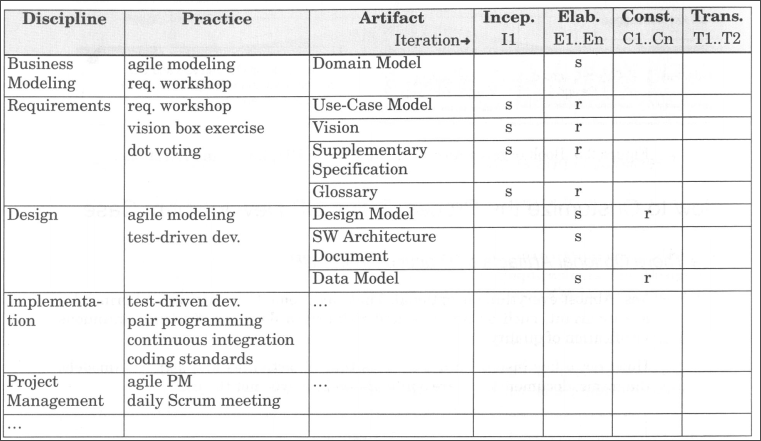
\includegraphics[scale=0.4]{2022-09-26-05_56_36.png}

\subsection{Phases of UP}
\begin{itemize}
  \item \textcolor{purple}{\textbf{\emph{Inception}}: Ceate a vision, scope, vague estimates and use cases.}
   \item \textcolor{purple}{\textbf{\emph{Elaboration}}: Create a refined vision, domain models, iterative implementation of core architecture, resolution of high risks, identification of most requirements and scope and more realistic estimates.}
   \item \textcolor{purple}{\textbf{\emph{Construction}}: Iterative implementation of remaining lower risk and easier elements, as well as preparation for deployment.}
   \item \textcolor{purple}{\textbf{\emph{Transition}}: beta tests and deployment}
\end{itemize} 

\subsection{CYNEFIN Framework}
  -------------- AGILE ---------------\newline
\begin{itemize}
  \item \textbf{Complex}: \textcolor{red}{P-S-R}\newline
\textbf{Probe, Sense, Respond}\newline
\textcolor{green}{Emergent Practice}
\item \textbf{Chaotic}: \textcolor{red}{A-S-R}\newline
\textbf{Analyze, Sense, Respond}\newline
\textcolor{green}{Novel Practice}\newline
  ------------- Classic --------------\newline
\item \textbf{Complicated}: \textcolor{red}{S-A-R}\newline
\textbf{Sense, Analyze, Resond}\newline
\textcolor{green}{Good Practice}
\item \textbf{Simple}:
\textcolor{red}{S-C-R}\newline
\textbf{Sense, Categorize, Respond}\newline
\textcolor{green}{Best Practice}\newline
  ------------------------------------
\end{itemize} 

\subsection{HERMES Swiss trash}
\textbf{Handbuch der Elektronischen Rechenzentren des Bundes, eine Methode zur
Entwicklung von Systemen}\newline
Category \& HERMES is a classical project method, once again this shows why Switzerland just fucking sucks in terms of software engineering as they clearly focus on the wrong method.\newline
\minipg{
benefits:\newline
\begin{itemize}
\item high standardization
\item many tools in many languages
\item national certification
\item embedding of scrum
\item good for public institutions
\end{itemize}
}
{
negatives:\newline
\begin{itemize}
\item very constricted, not many freedoms
\item four phases, which are rather short
\item not relevant outside of Switzerland, yay WHY EVEN PROPOSE THIS CRAP THEN?!
\item HERMES complicates projects...
\end{itemize}
}[0.2,0.3]

\subsubsection{Phases} 
HERMES knows 4 phases:\newline
\begin{itemize}
  \item \textcolor{red}{Initialization} \textcolor{teal}{Goals, Requirements, Variants}
  \item \textcolor{red}{concepts} \textcolor{teal}{System requirements, Details, System architecture, prototypes}
  \item \textcolor{red}{Realization} \textcolor{teal}{Detail-specifications, system developed}
  \item \textcolor{red}{Introduction} \textcolor{teal}{system activated}
\end{itemize}
\textcolor{red}{The project manager is only free to operate within these phases, each change of phase needs to be approve by the \textbf{"Lenkungsausschuss"}, which is essentially a group of all parties with interest in this project.}

\section{Elements of a Project}
\begin{itemize}
\item \textcolor{purple}{Finances}\newline
  \begin{itemize}
  \item \textcolor{black}{Return of Investment}
  \item \textcolor{black}{Less Spending}
  \item \textcolor{black}{More Income}
  \end{itemize} 
\item \textcolor{purple}{Compliance}\newline
  \begin{itemize}
  \item \textcolor{black}{Compliance with Law}
  \item \textcolor{black}{Compliance with standards}
  \item \textcolor{black}{Compliance with soft law}\newline
    law based on public opinion
  \end{itemize} 
\item \textcolor{purple}{Agility}\newline
  \begin{itemize}
  \item \textcolor{black}{Fast Processes}
  \item \textcolor{black}{Flexible Structures}
  \item \textcolor{black}{Fast Time to Market}
  \end{itemize} 
\item \textcolor{purple}{Quality}\newline
  \begin{itemize}
  \item \textcolor{black}{Gaining an Image}
  \item \textcolor{black}{Reliability}
  \item \textcolor{black}{Data-Hygene}
  \end{itemize} 
\end{itemize} 

\section{ROI Return Of Investment}
The ROI is the time it takes for the project to return the amount of money that was spent on creating it.\newline
In other words, at what timeframe are you even with the costs that you have spent? 

\subsection{Business Case}
This is the comparison between all cases that could happen within a project:\newline
\textcolor{orange}{Normal Case, Best Case, Worst Case, Small Case, Outsourcing Case, ...}\newline
\textcolor{teal}{Note that with the Prince2 Method, you will always have to compare these cases for each project.} 

\subsection{Financing} 
\begin{itemize}
\item \textcolor{purple}{Internal Projects}\newline
  With internal projects there usually isn't a problem with financing, as the money is there either way, otherwise the project wouldn't have been started, usually the amounts are given out per phase.(with classic methods)
\item \textcolor{purple}{External Projects}\newline
  This is where the problems lay, customers don't want to pay you for work that is not yet done, but at the same time, you also need an income for the time where you are working on the project, and it could very well mean that you will not earn any income for half a year or more, depending on how big the project is.\newline
  Usually this is why a lot of companies rely on monthly contract payouts with an end-sum for the finished project.\newline
  Agile projects have an additional advantage, as they can simply charge for each function point that they have implemented.
\end{itemize} 

\subsection{Contracts}
Contracts in Switzerland are made in 3 ways:\newline
\textcolor{purple}{written}: \newline
Usually done for formal settings, including business relations <- most important for this \newline
\textcolor{purple}{oral}:\newline
Usually between friends or first part of a contract -> later turned to written contract\newline
\textcolor{purple}{Concluded}:\newline
A contract that is kinda obvious: place the items that you want to buy in a grocery shop on the tray.

\subsection{"Werkvertrag" vs "Einfacher Vertrag"} 
The simple difference is that the "Werkvertrag" requires the end result itself and has a fixed price and a fixed timeframe.\newline
Any changes to the contract are made by both parties, and there is no involvement of law.\newline
With the "Einfacher Vertrag", the work itself is sold and therefore the price is based on that work, it also means that any delays are solely the risk of the customer, as you essentially just work for them.\newline
\textcolor{red}{TDLR: A "Werkvertrag" is selling a product. While an "Einfacher Vertrag" is being a contractor.}

\section{Risks and Opportunities}

\subsection{Risk Analysis}
Risk Analysis has 5 stages: \newline
\begin{itemize}
\item \textcolor{purple}{Identify Risks}
  \begin{itemize}
  \item \textcolor{black}{Impact Analysis}\newline
    Check which sections of the project are often impacted and choose risks based on it
  \item \textcolor{black}{Potential Dangers}\newline
    Choose potential dangers from a catalog
  \item \textcolor{black}{Identify Weak-Points}\newline
    Based on experience, choose dangers that might impact this project
  \item \textcolor{black}{Combination of the above}
  \end{itemize} 
\item \textcolor{purple}{Categorize Risks}
  categorize the risk based on the likelyhood of appearing and the amount of damage it does when it appears
\item \textcolor{purple}{Rank Risks}\newline 
  Create a ranking based on the previous categorization, making it possible to tackle the big risks first.\newline
  If risks are considered to not be big enough, they are under the so called \textbf{acceptance line}.
\item \textcolor{purple}{Use Risk Strategies}\newline 
\begin{itemize}
\item Risk Mitigation Implementation of safeguards in order to
\item eliminate vulnerabilities or block threats
\item Risk Assignment / Risk Transferring \newline
  purchasing insurance or outsourcing. Transfer the cost of risk to other entity
\item Risk Acceptance Doing nothing as cost/benefit would be low
\item Risk Deterrence auditing, cameras, security guards, warnings, etc
\item Risk Avoidance Not using the system associated with the risk
\item Risk Rejection Simply ignore risk \textcolor{red}{without cost/benefit analysis!}
\item Residual Risk A countermeasure might not fully eliminate a risk\newline 
  This is the remaining risk that we have decided to accept.
\item \textcolor{purple}{Implement Counter Measures}
\end{itemize} 
\end{itemize} 

\subsection{GAMP5}
This standard was made in the pharma industry and can be used in IT, apparently. <- F to doubt\newline
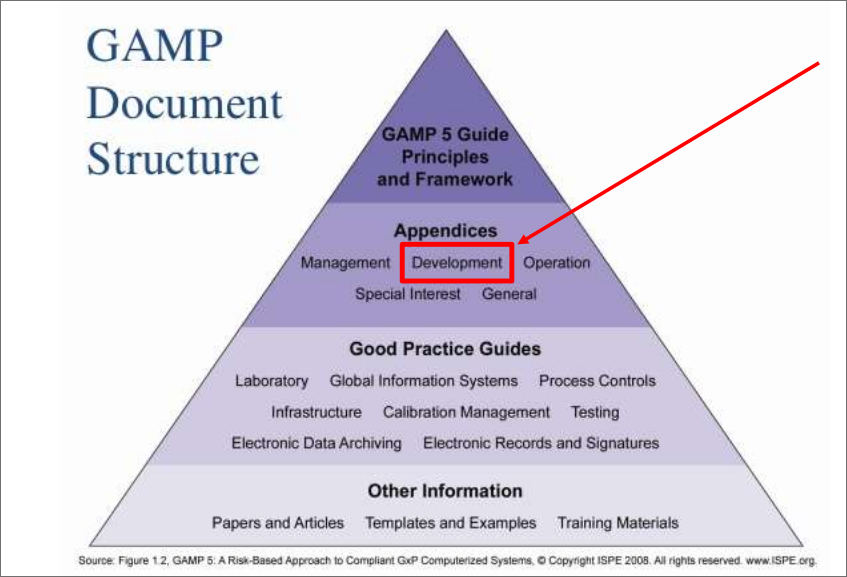
\includegraphics[scale=0.3]{2023_01_09_05_00_31.png}

\subsection{SWOT Analysis}
A very wide adopted system to balance opportunities and risks\newline
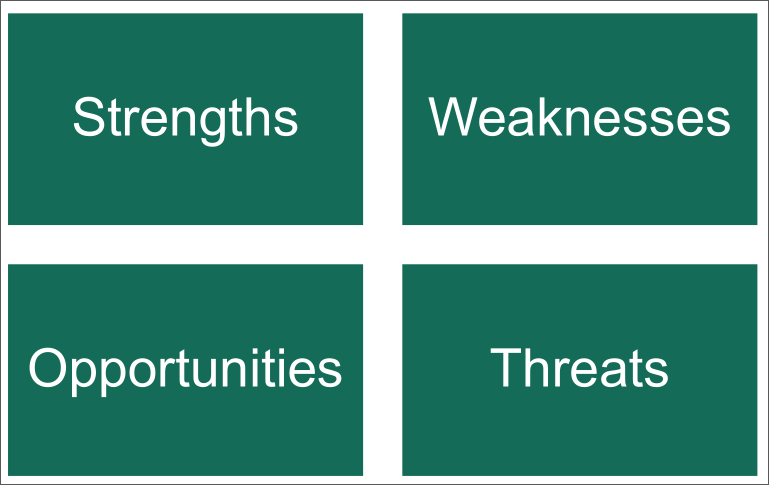
\includegraphics[scale=0.3]{2023_01_09_05_02_01.png}

\section{Quality Assurance}

\subsection{Security}
\subsubsection{CIA triad}
The primary goal of Security infrastructure:\newline
\begin{itemize}
  \item \textcolor{red}{C}\textcolor{blue}{onfidientiality:} prevention of unauthorized access to data\newline
{no matter if the data is \textcolor{red}{in transit, in storage or in process}}\newline
{Usually done with \textcolor{red}{encryption and access control}}
\item \textcolor{red}{I}\textcolor{blue}{ntegrity:} prevention of unauthorized alteration of data\newline
{\textcolor{green}{Data integrity:} data is complete, consistent and accurate}\newline
{\textcolor{green}{System integrity:} System only does what it was intended to do}\newline
{Usually  done with \textcolor{red}{hash verification, intrusion detection}}
\item \textcolor{red}{A}\textcolor{blue}{vailability:} Systems should be accessible at all times\newline
{Usuall done with \textcolor{red}{Redundancy, backups}}
\end{itemize} 

\subsubsection{NonRepudation \& Accountability}
Nonrepudation ensures that every action can be traced to the actual source\newline
This prevents attackers from covering their actions.\newline
Accountability ensures that every being is responsible for their actions.\newline
E.G. Nonrepudation ensures Accountability.\newline
Usually done with certificates, session identifiers, logs, etc

\subsection{Constructive vs Analytical}
Software assurance always relies on both the analytical aspect, where you simply check if the code or in general your project works as intended without flaws or vulnerabilities. \newline
Meanwhile the constructive part ensure that it can't even get there, for example with unit tests, or proper development strategies etc. 

\subsection{Continuous Delivery}
This is simply the continuous shipment of the state of the project to the customer. \newline
It ensures that the customer is always up to date with the current project and directly influence the development, making sure that the endproduct is perfectly fit for the job.\newline
\textcolor{red}{As once can see, this is where the agile aspect shines, since you can just show each function that got implemented since the last time you have shown the product to the customer.\newline
AND, you might even have backup implementations in case the customer would like something else!!}

\subsection{Change Request -> Classical}
With classical methods, changes have to be approved. This is because you already planned everything and now you need to reduce either scope, increase the time needed, or increase the cost. \newline
This is another reason why IT does NOT benefit from classical methods. Changes are often sudden and spontaneous. \newline
\textcolor{purple}{It is important to write it as a request, not as an ultimatum, in other words, use "due to sudden circumstances", instead of "we need this or else".\newline
However, it is necessary to clearly define the outcomes of both accepting the change request and declining the change request, as this is critical for the decision.}\newline
In general the change request is made this way to avoid invoking decisions and language based on feeling, which might casue infighting.\newline
\textcolor{red}{A change request always needs to include the new scope, time and budget!}

\subsection{Change in Agile}
Since agile is the better variant either way, the change can just be added as another user story, or just edit an existing one.\newline
The user story can then be ranked as the other ones and worked on accordingly. \newline
So Fucking Easy. 

\subsection{SixSigma} 
\begin{itemize}
\item \textcolor{red}{\textbf{Define Measure Analyze Improve Control}}
\item \textcolor{orange}{Mathematical Model to measure and optimize processes}
\item \textcolor{orange}{independent of process or sector}
\item \textcolor{orange}{Shows how KPI is measured and how the process can be optimized by it}
\end{itemize}

\subsubsection{SixSigma Define}
\textcolor{red}{SIPOC -> Supplier - Input - Process - Output - Customer}\newline
\textcolor{orange}{SIPOC is the journey from the supplier to the customer, \newline
it defines what happens where in order to later on improve the workflow}\newline
\textcolor{red}{KOMY -> Key Output Measurement}\newline
\textcolor{orange}{KOMY is the formula that converts all input values to one output value.}

\subsubsection{SixSigma Measure} 
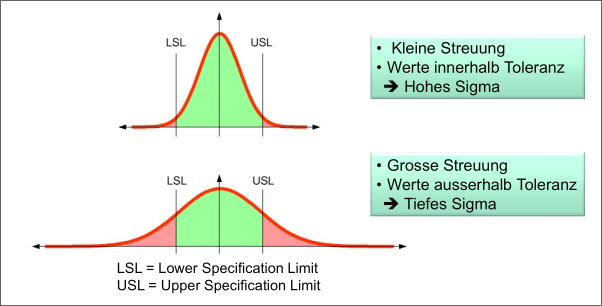
\includegraphics[scale=0.4]{2022-10-31-11_20_10.png}

\subsubsection{SixSigma Improve} 
\textcolor{orange}{In order to improve you need 3 things:}\newline
\begin{itemize}
\item \textcolor{teal}{Knowledge and Skills}
\item \textcolor{teal}{Tools}
\item \textcolor{teal}{Mentality and Behavior}
\end{itemize}

\subsection{5 Aspects of Data Quality}
\begin{itemize}
\item \textcolor{purple}{Consistency}
\item \textcolor{purple}{Validity}
\item \textcolor{purple}{Completeness}
\item \textcolor{purple}{Correctness}
\item \textcolor{purple}{Actuality -> up-do-date data}
\end{itemize} 
\textcolor{teal}{In general, make sure data is correct the first time, fixing data afterwards can be very expensive and painful, especially if your work was done based on the previous data that has now been confirmed to be wrong!}\newline
Avoid "Disconnected Silos", aka void choosing data that comes from one source only, choose many!

\section{testing}

\subsection{Requirements for Tests}
\begin{itemize}
\item \textcolor{purple}{Reproducability}
\item \textcolor{purple}{Planability}
\item \textcolor{purple}{economical impact}
\item \textcolor{purple}{Risk and Responsibility reduction}
\end{itemize} 

\subsection{Types of Tests}
\begin{itemize}
\item \textcolor{purple}{static}\newline
  These are tests that do not affect the running program.\newline
  Ex. static code analysis.\newline
  \begin{itemize}
  \item \textcolor{black}{Inspection}
  \item \textcolor{black}{Walkthrough}
  \end{itemize} 
\item \textcolor{purple}{dynamic}\newline
  These are tests that are done during runtime of the program\newline
  \begin{itemize}
  \item \textcolor{black}{Functional test}
  \item \textcolor{black}{DataFlow test}
  \end{itemize} 
\end{itemize} 

\subsection{Test Hierarchy} 
\begin{enumerate}
\item \textcolor{purple}{Unit test}
\item \textcolor{purple}{Integration Test}
\item \textcolor{purple}{System Test}\newline
  Usually a whitebox test\newline
  --------------------- end of IT specific
\item \textcolor{purple}{Final Use test (before customer accepts product)}\newline
  Usually a blackbox test, aka the entire program is considered to be as one.
\item \textcolor{purple}{Usage by customer (after customer accepted product)}
\end{enumerate} 

\subsection{General types of tests}
\begin{itemize}
\item \textcolor{purple}{Positive Test}\newline
  Here the program is testes whether or not it works with the intended inputs
\item \textcolor{purple}{Negative Tests}\newline
  Here the program is tested against nonsense input or deliberate wrong input
\end{itemize} 

\subsection{Testing in classical vs agile}
Classical has fixed timestamps where proper testing is done, again this is NOT FUCKING POSSIBLE IN IT!\newline
So the only solution is agile, where we test anytime and all the time.\newline
A good example is CI pipelines which run everytime you implement any feature, it makes sure that everything before this feature still works, and if you did your job properly, that means you also implemented tests which now also are going to be run by the pipeline!\newline
\textcolor{purple}{The agile format does not have a specific timestamp to test! They test all the time!}

\subsection{Structure of a Bug/Error Report}
\begin{enumerate}
\item \textcolor{purple}{Problem Description}
\item \textcolor{purple}{Identification}
\item \textcolor{purple}{Classification}
\end{enumerate} 

\subsection{Configuration Management}
\minipg{
Why?\newline
\begin{itemize}
\item \textcolor{purple}{Guarantee of quality}
\item \textcolor{purple}{Proper Delivery}
\item \textcolor{purple}{Logs of Development timeline}
\item \textcolor{purple}{Structuring of Changes}
\item \textcolor{purple}{Overview of changes and its processes}
\item \textcolor{purple}{Error Corrections and its consequences}
\end{itemize} 
}{
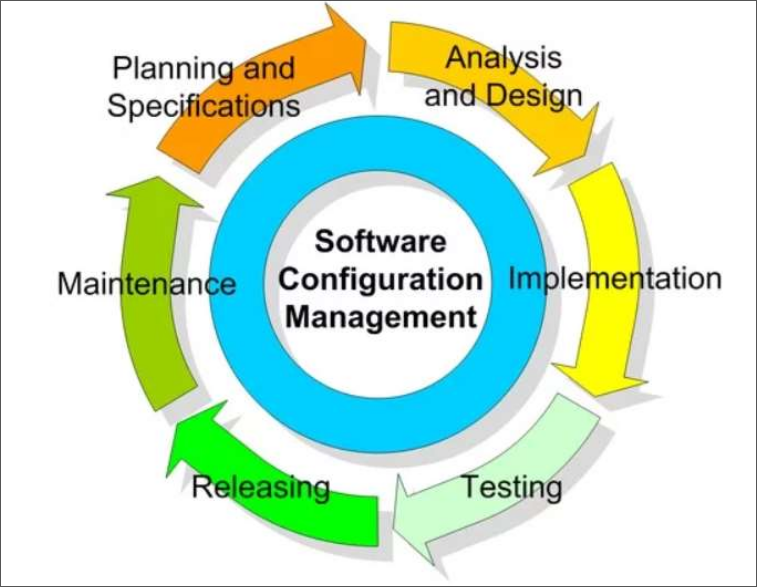
\includegraphics[scale=0.25]{2023_01_09_05_54_00.png}
}[0.25,0.25]
small note, apparently configuration also includes testing, not sure why that is called configuration then...

\section{Agile}
\subsection{Agile Manifesto}
\begin{itemize}
\item \textcolor{purple}{Individuals and Interactions over processes and tools}\newline
  Let the devs choose the tools, but make sure you have the right devs!
\item \textcolor{purple}{Functional Software over complete documentation}\newline
  If the software works you can always go back and add documentation, but documentation for broken software is useless!
\item \textcolor{purple}{Cooperation with customer over Contract negotiations}\newline
  We do not need to follow a strict plan, we can always renegotiate!
\item \textcolor{purple}{Reacting to change over following a plan}\newline
  If the customer wants a change then the customer wants a change, the plan be damned. 
\end{itemize} 

\subsection{Principles}
\begin{itemize}
\item \textcolor{purple}{Highest priority is a content customer}\newline
\item \textcolor{purple}{Big changes are always welcome, even in the right before the end}
\item \textcolor{purple}{Value working software with small steps -> function points and user stories}
\item \textcolor{purple}{Sector Experts and developers need to work together on a daily basis}\newline
  DSTAM -> Daily Standup Meeting (GEIL)
\item \textcolor{purple}{Create Projects around motivated individuals and give them the environment they need to work}
\item \textcolor{purple}{The most effective method to relay information if from person to person}\newline
  Hence the experts working with devs thing
\item \textcolor{purple}{The best work is done by self-created teams}
\item \textcolor{purple}{Reflection within timeframes in order to improve effectiveness}
\item \textcolor{purple}{Keep a constant tempo}\newline
  Do not overburn the team, as it will otherwise slow down at some point!
\item \textcolor{purple}{Value excellence -> keep your devs motivated, give them free room, let them take time off if they are overwhelmed}
\item \textcolor{purple}{Split not completed work into extremely small pieces in order to properly rank the importance of work}
\end{itemize} 
\textcolor{red}{There is one big downside for companies with this: the cost, scope and timeframe is not always clear with agile.\newline
This leads to the company needing to allocate more than it might want to.}\newline
In general agile is not compatible with the old way of thinking, since agile gives power to dev directly and takes it away from managers and bosses.\newline
This will clash with the "I AM THE BOSS" mentality.


\subsection{Notable Signs for Agile}
\begin{itemize}
\item \textcolor{purple}{Inspect and Adapt}\newline
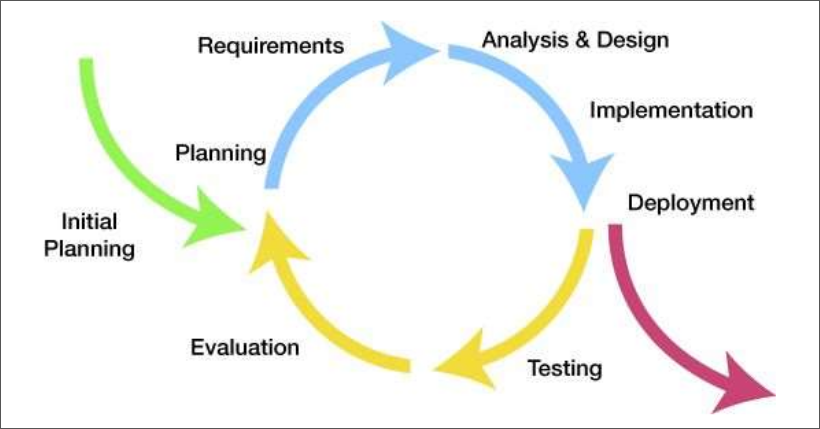
\includegraphics[scale=0.3]{2023_01_09_06_24_58.png}
\item \textcolor{purple}{Transparency}\newline
\begin{itemize}
\item \textcolor{black}{Information is kept simple and available to everyone}
\item \textcolor{black}{Quality and working software are signs for progress}
\item \textcolor{black}{No hidden agenda or alternative progress checking}
\item \textcolor{black}{Visualization of data}
\end{itemize} 
\item \textcolor{purple}{Self Organization}
\item \textcolor{purple}{(TimeBoxing) not really but the lecture materials said so}\newline
\end{itemize} 

\subsection{TimeBoxing vs FunctionBoxing}
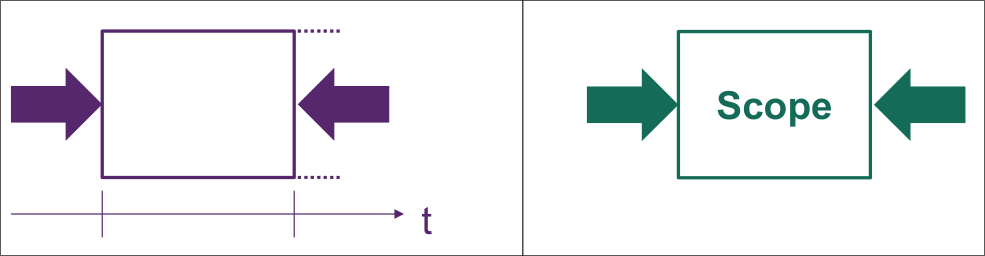
\includegraphics[scale=0.3]{2023_01_09_06_28_45.png}\newline
\begin{itemize}
\item \textcolor{purple}{Time Boxed}\newline
\begin{itemize}
\item \textcolor{black}{Fixed time length for sprint}
\item \textcolor{black}{not finished work pushed to next sprint}
\item \textcolor{black}{Employees are shielded from outside influence}
\end{itemize} 
\item \textcolor{purple}{Function Boxed}
\begin{itemize}
\item \textcolor{black}{fixed scope for sprint, all work will be finished}
\item \textcolor{black}{flexible time length}
\item \textcolor{black}{Employees are shielded from outside influence}
\end{itemize} 
\end{itemize} 

\subsection{User Stories}
User stories are brief needs that are written from the pov of the user.\newline
Meaning that the user states that they would like to do x with y functionality with your program.\newline
Structure:\newline
\textcolor{red}{As a \_\_\_\_\_\_, I can \_\_\_\_\_\_\_ my \_\_\_\_\_\_\_\_. \newline
As a "user", I can "backup", my "hard-drive".}

\subsubsection{INVEST-Criteria for User Stories}
\begin{itemize}
\item \textcolor{purple}{Independent}: each user story is independent from another
\item \textcolor{purple}{Negotiable}: each user story can be discussed -> potentially modified or removed
\item \textcolor{purple}{Valuable}: is of use to some user
\item \textcolor{purple}{Estimable}: time or scope needs to be clear
\item \textcolor{purple}{Small}: work should be pos-x compliant for maximum split
\item \textcolor{purple}{Testable}: needs to be testable in order to be considered done
\end{itemize} 

\subsection{SCRUM}
Note, scrum is not strictly agile, it is often considered to be bastardization of it.\newline
\begin{itemize}
\item \textcolor{purple}{Based on fixed time sprints}
\item \textcolor{purple}{Different Roles}
\item \textcolor{purple}{Artifacts for documents}
\item \textcolor{purple}{Ceremonies}
\end{itemize} 

\subsection{Categorization of Work}
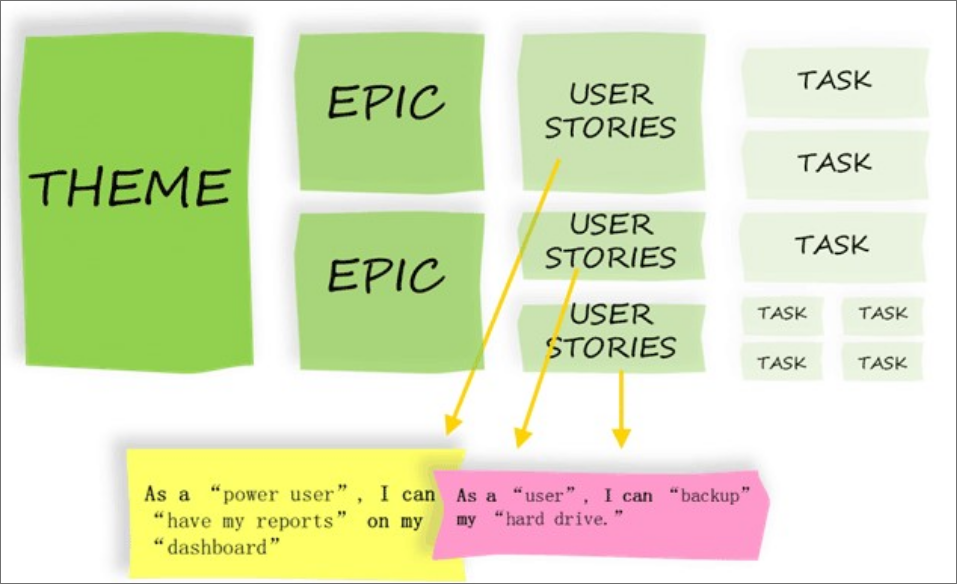
\includegraphics[scale=0.2]{2023_01_09_07_07_49.png}

\subsubsection{Roles in SCRUM}
\begin{itemize}
\item \textcolor{purple}{Product Owner}\newline
  The person who came up with the idea
\item \textcolor{purple}{Development Team}\newline
  The team that implements the idea
\item \textcolor{purple}{Scrum Master}\newline
  The person who will manage the interaction
\end{itemize} 

\subsubsection{Artifacts in SCRUM}
\begin{itemize}
\item \textcolor{purple}{Product Backlog}
\item \textcolor{purple}{Sprint Backlog}
\item \textcolor{purple}{Increment}
\end{itemize} 

\subsubsection{Ceremonies in SCRUM}
\begin{itemize}
\item \textcolor{purple}{Sprint}: 2 - 4 weeks
\item \textcolor{purple}{Sprint Planning}: < 4-8 hours\newline
  Product owner specifies user stories, prioritizes them and puts all user stories in the product backlog.\newline
  The dev team then puts the user stories with new prioritization to the sprint backlog.\newline
  Note that only a specific amount of user stories will be included in the sprint backlog.
\item \textcolor{purple}{Sprint Review}: < 2-4 hours\newline
  showcase the work to the project owner. \newline
  Done after sprint, entries from product backlog are discussed.
\item \textcolor{purple}{Sprint Retrospektive}: 1.5 to 3 hours\newline
  review the sprint, and improve on it
\item \textcolor{purple}{Daily Scrum}: < 15min\newline
  simple interaction with other teams to clarify the current state.\newline
  Entries from the sprint backlog are discussed.
\end{itemize} 

\subsubsection{SCRUM Sprint}
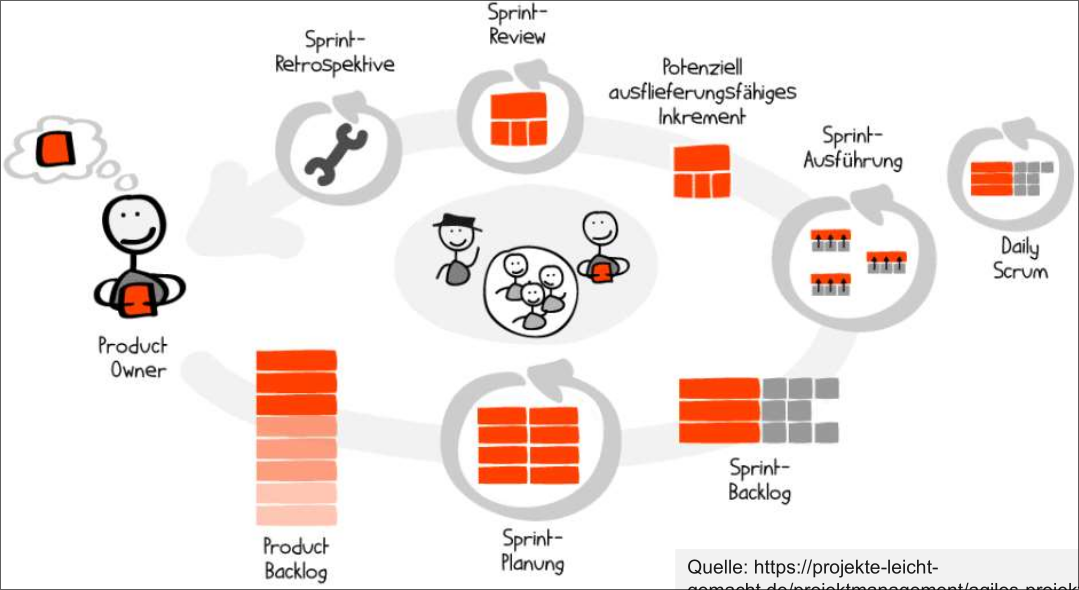
\includegraphics[scale=0.3]{2023_01_10_01_09_48.png}

\subsection{Kanban (NOT AGILE...)}
\begin{itemize}
\item \textcolor{purple}{represents the IS-State}
\item \textcolor{purple}{visualize work}
\item \textcolor{purple}{sets limits on what one can work}
\item \textcolor{purple}{Entire work split into rough patches}
\item \textcolor{purple}{React to prognosis}
\end{itemize} 
\textcolor{teal}{The name kanban is from the chinese language and means look-at (the) board}\newline
\textcolor{teal}{Kanban revolutionized the automobile industry with toyota}\newline
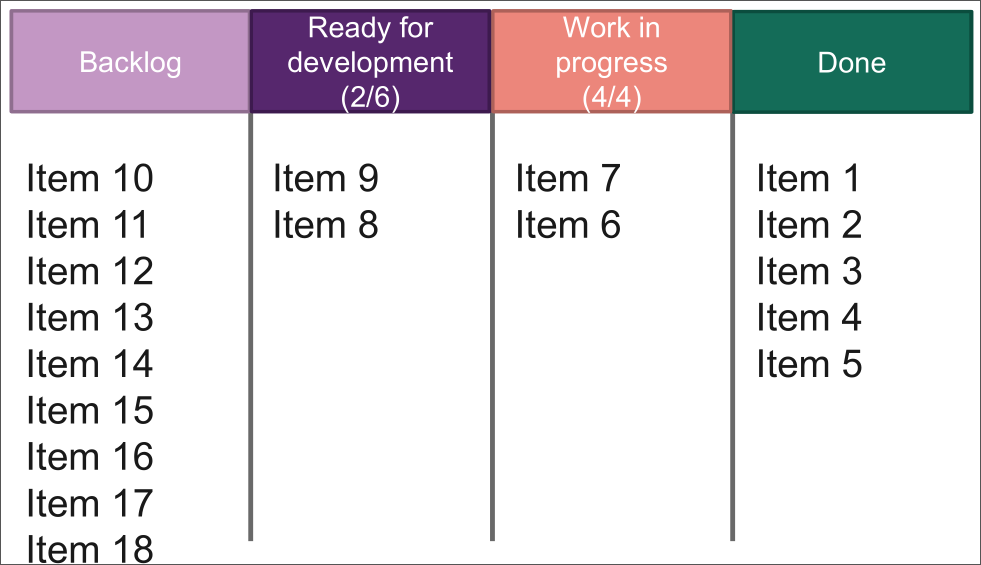
\includegraphics[scale=0.3]{2023_01_10_12_19_29.png}\newline
Technically there is scrumban, which is a bastardized mix of the two.

\section{Communication}
\subsection{Stakeholder}
\begin{itemize}
\item \textcolor{purple}{Every party that is interested in the project is considered a stakeholder}
\item \textcolor{purple}{Stakeholders represent different group of needs}
\item \textcolor{purple}{Project manager should include stakeholder in the development of the project}
\item \textcolor{purple}{continuously update information for stakeholders and inform them}
\end{itemize} 

\subsubsection{Finding Stakeholders}
\begin{enumerate}
\item \textcolor{purple}{Who works on the project and who provides the resources?}
\item \textcolor{purple}{Who can influence the project?}
\item \textcolor{purple}{Who is affected by the project?}
\item \textcolor{purple}{Who can influence the success of the project}
\item \textcolor{purple}{Who will be the user of the project?}
\item \textcolor{purple}{Who MUST be involved?}
\end{enumerate}
\textcolor{red}{For the module, the project team is not considered a stakeholder, however according to the 6 questions it definitely is a stakeholder.}

\subsubsection{Interests and Influence of Stakeholders}
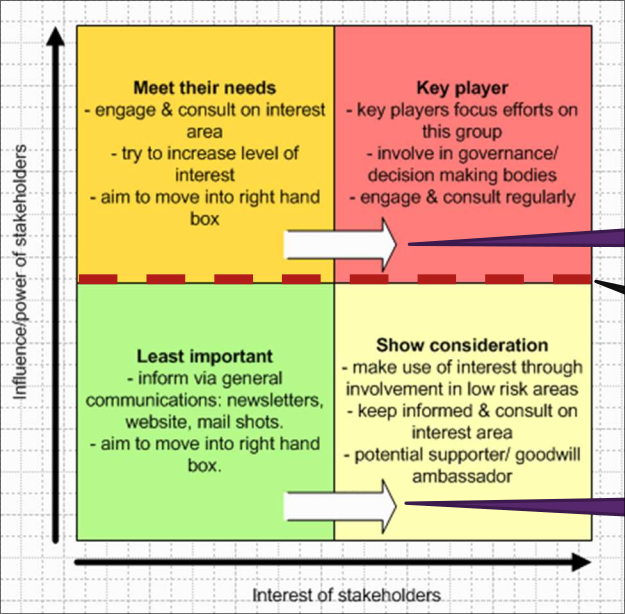
\includegraphics[scale=0.3]{2023_01_10_12_27_49.png}\newline
Depending on the influence and interest of the stakeholder, make sure you give them appropriate attention and work with them.\newline
\textcolor{red}{Note, do not just let stakeholders cross the red line without reason.}

\subsubsection{Conflicts and Harmony with stakeholders}
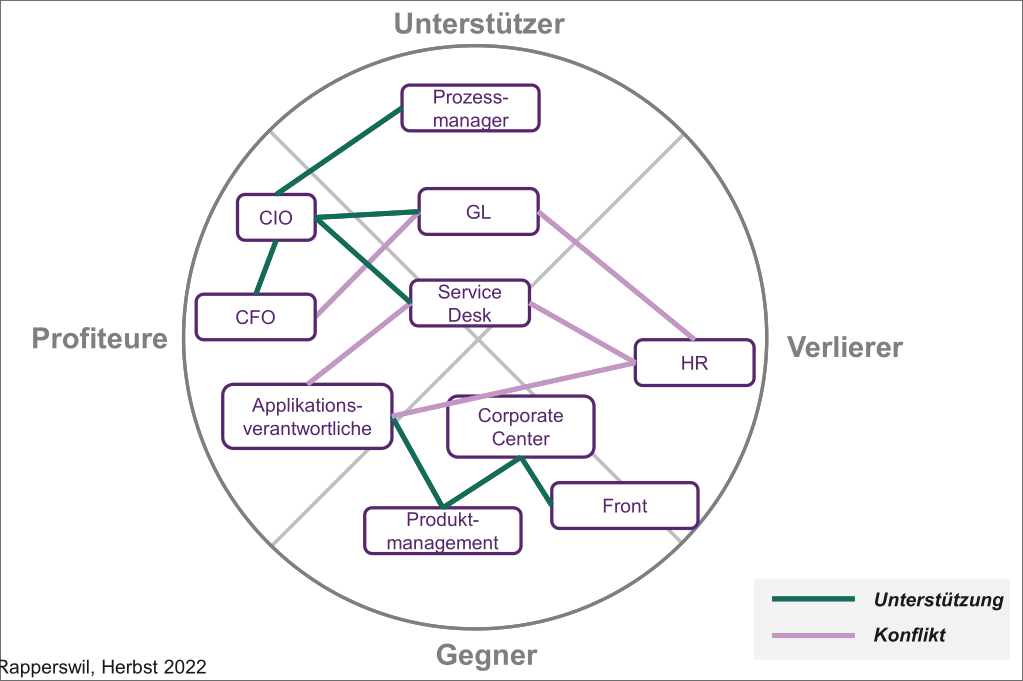
\includegraphics[scale=0.3]{2023_01_10_12_40_44.png}

\subsection{Leadership}
Leadership is simply the act of coordination within a project.\newline
As expected, there are multiple variants of leadership, some allow the team-members more autonomy, some less.\newline
Note that for agile methods, autonomy is a requirement.\newline
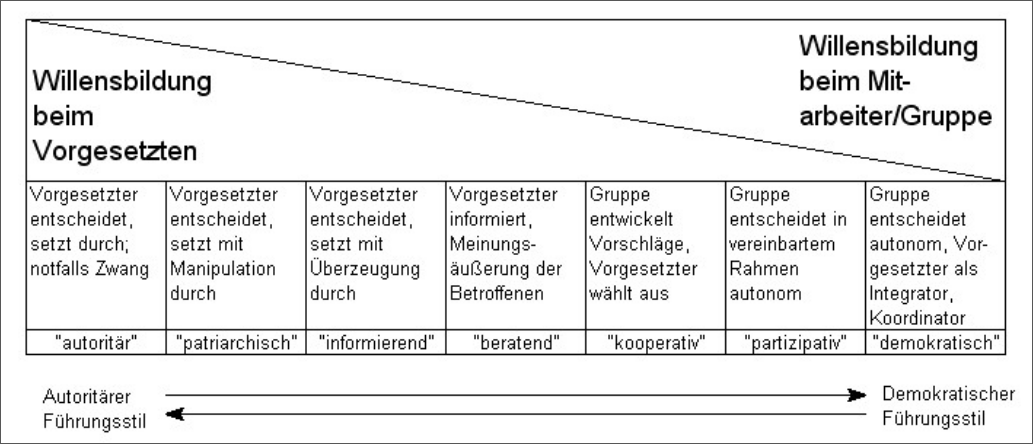
\includegraphics[scale=0.3]{2023_01_10_12_42_34.png}\newline
\textcolor{teal}{This means however, that not everyone can fit into the agile development style, as they require more strict guidelines on what, how and when.} 

\subsubsection{Leadership Rhythm} 
This simply states how many times you: \textbf{receive information, consider the information, make a decision based on the information and check the results of it}.\newline
Keep this rhythm as low as possible, but increase it if challenges appear.

\subsection{Communication Matrix}
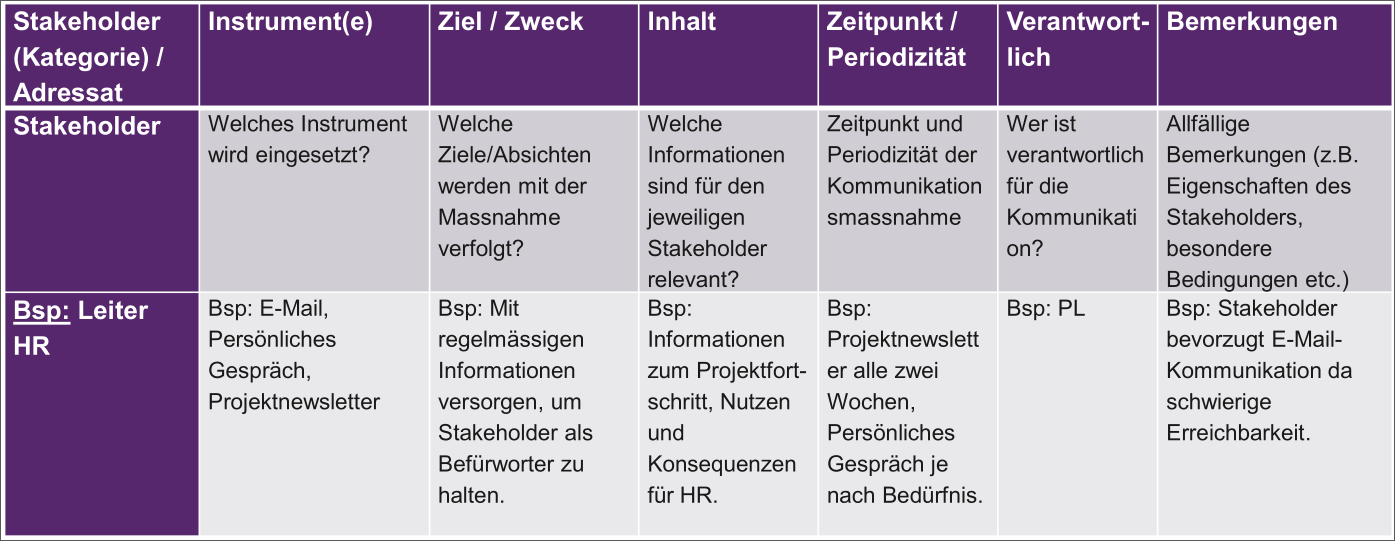
\includegraphics[scale=0.28]{2023_01_10_12_51_33.png}\newline
Apparently you should always define who will communicate with who clearly.\newline
But if you remember the agile methods, then you notice that this does not always make sense.\newline
For communication between customer and your team it might make sense, since the team should not be bothered with bullshit, instead they should be talking to people who are involved with the project directly.\newline
Making too many assumptions about who is useful would make this whole ordeal waterfall again.....
 
\subsection{Quality over Quantity}
\begin{itemize}
\item \textcolor{purple}{Communicate only when necessary}
\item \textcolor{purple}{Leave irrelevant information out}
\item \textcolor{purple}{Do not involve stakeholders that do not need this information}
\end{itemize}

\subsection{Schulz von Thun}
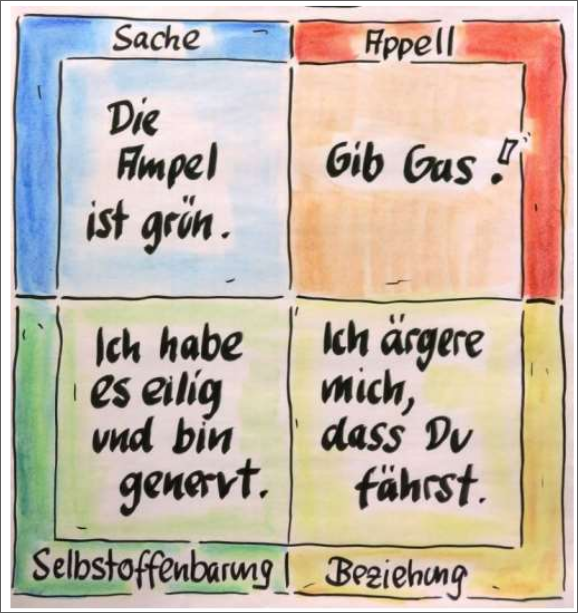
\includegraphics[scale=0.3]{2023_01_10_12_55_27.png}\newline
With communication, we have one obvious problem. Sometimes we will aggravate someone without intending to do so.\newline
It is therefore important to at least try to keep it on the \textbf{informational ("sachlich")} level.\newline
Other forms of communication are not suitable for cooperation inside a project. 

\subsection{Marketing}
\textcolor{purple}{It is more than just advertising}\newline
\begin{itemize}
\item \textcolor{black}{Leads the kick-off for the project}
\item \textcolor{black}{Included in planning}
\item \textcolor{black}{Sets the initial targets and proposition for stakeholders}
\item \textcolor{black}{Relays information on project status to stakeholders}
\item Gives recognition to the project team after project end 
\item shows use case and advertises product at the end of the project
\end{itemize} 
\textcolor{teal}{The project manager as \textbf{ambassador}, in other words, the most valuable skill for companies in project managers is often the presentation of the project to others, including but not limited to the customer or other stakeholders.}\newline
Once again, note here that the project manager is much more involved in this role with the classical approach rather than the agile one.\newline
Most stakeholders would interact with the team directly in an agile environment. 

\subsection{Documentation}
We differentiate between 2 types of documentation:\newline
\begin{itemize}
\item \textcolor{purple}{static documentation}\newline
  These are documentation that represent the results of the project and are therefore no longer needed when the project has eneded.\newline
  These docs will be archived.\newline
  \begin{itemize}
  \item \textcolor{black}{Phase independent documentation}
  \item \textcolor{black}{Phase dependent documentation}
  \end{itemize} 
\item \textcolor{purple}{dynamic documentation}\newline
  These docs are updates regularly and will also be "shipped" with the product.\newline
  \begin{itemize}
  \item \textcolor{black}{user documentation}
  \item \textcolor{black}{maintenance documentation}
  \item \textcolor{black}{usage documentation}
  \end{itemize} 
\end{itemize} 
\textcolor{teal}{Note, once again this is made for the classical approach, as can be seen by the mention of the word "phases", agile does not really care about the first part, bar the user stories.}

\section{Cooperation and Solutions}

\subsection{Techniques for finding solutions}
\begin{itemize}
\item \textcolor{purple}{brainstorming}\newline
  \begin{itemize}
  \item \textcolor{orange}{Protocol leader writes down all ideas}
  \item \textcolor{orange}{Discussion Leader formulates the problem and oversees discussion}
  \item \textcolor{orange}{Criticism is forbidden -> analysis after brainstorming}
  \item \textcolor{black}{ALL ideas are welcome and will be written down}
  \item \textcolor{black}{broad spread of ideas}
  \item \textcolor{black}{Team should be diverse, but not with too many differences in hierarchy}
  \item Combine and expand existing ideas
  \end{itemize}
  \textcolor{red}{Brainstorming is good for creativity, but not when competency is required!}
\item \textcolor{purple}{Method 635}\newline
  \begin{itemize}
    \item \textcolor{black}{\textbf{6 participants and 6 papers}}
    \item \textcolor{black}{each participant writes down \textbf{3 ideas} on their own paper}
  \item \textcolor{black}{after that give the paper to the next person}
  \item \textcolor{black}{That person will then expand the paper with another 3 ideas that are based on the previous ones, or expand the previous ones}
  \item \textcolor{black}{This is \textbf{repeated 5 times}}
  \item Time for each round: 5min, 6min, 7min, 8min, 9min, 10min
  \end{itemize} 
\item \textcolor{purple}{Morphological Box}
  With this method you try to \textbf{split the problem into smaller problems}, then you will try to find solutions for each underlying problem.\newline
  At the end you will give each person a pen and let them choose the "path" that will lead to their solution.\newline
  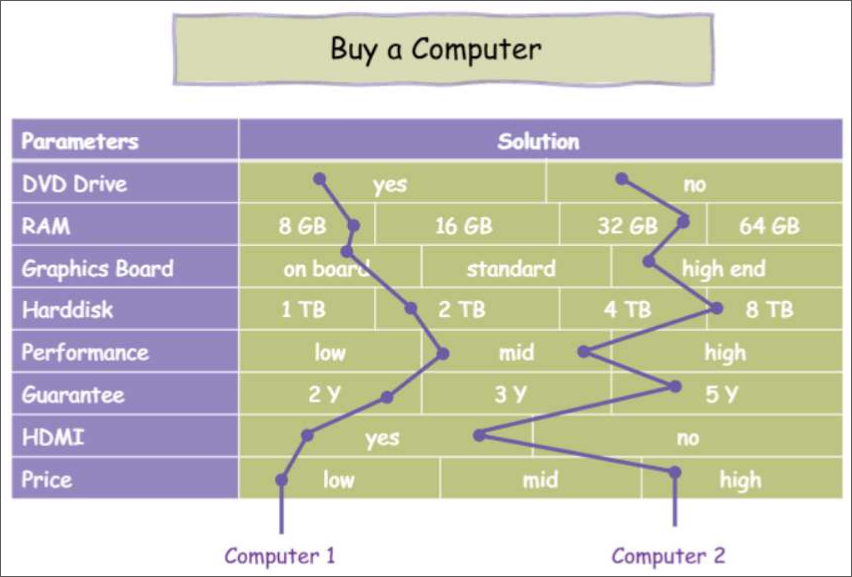
\includegraphics[scale=0.3]{2023_01_10_01_29_58.png}
\end{itemize} 

\subsection{Techniques for evaluating solutions}
\begin{itemize}
\item \textcolor{purple}{Value analysis}\newline
  \begin{itemize}
  \item \textcolor{orange}{List Criteria}
  \item \textcolor{orange}{Weight Criteria}
  \item \textcolor{black}{Each solution will be evaluated for each criteria}
  \item \textcolor{black}{sum up the points for each solution -> most points wins.}
  \end{itemize} 
  \textcolor{teal}{With small point differences you might find some other things that will make the difference...}
\item \textcolor{purple}{Decision Tree}\newline
  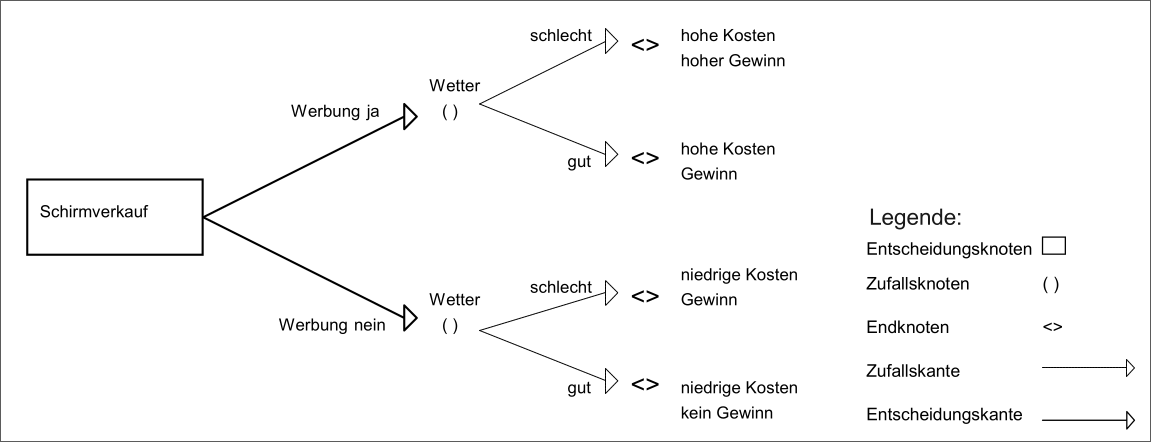
\includegraphics[scale=0.3]{2023_01_10_01_37_59.png}
\end{itemize} 

\subsection{Meeting Techniques}
Questions before the meeting:\newline
\begin{itemize}
\item \textcolor{black}{Is the meeting necessary? LMAO}
\item \textcolor{black}{Are the goals clear?}
\item \textcolor{black}{Who needs to be present?}
\item \textcolor{black}{Do the participants even have time?}
\item What should be the end result for every participant?
\item What are the dependencies with the project?
\item What is the order of items to be discussed?
\end{itemize} 

\subsubsection{How to act as Meetingleader}
\begin{itemize}
\item \textcolor{black}{specify a protocol writer}
\item \textcolor{black}{stay within the timeframe!}
\item \textcolor{black}{moderate the meeting not lead it}
\item \textcolor{black}{never be personal}
\item stop any distractions
\item record decisions, activities and appointments
\end{itemize} 

\subsubsection{Participants in the meeting}
As a leader you need to be prepared for everything.\newline
You might have participants who are shy, and never really express themselves, even when it would be necessary for them to do so.\newline
However, you might also have a rainbow dash, who can't keep her mouth shut:P. \newline
In other words, you need to make sure that the tone and atmosphere is civil and helpful for the project.\newline
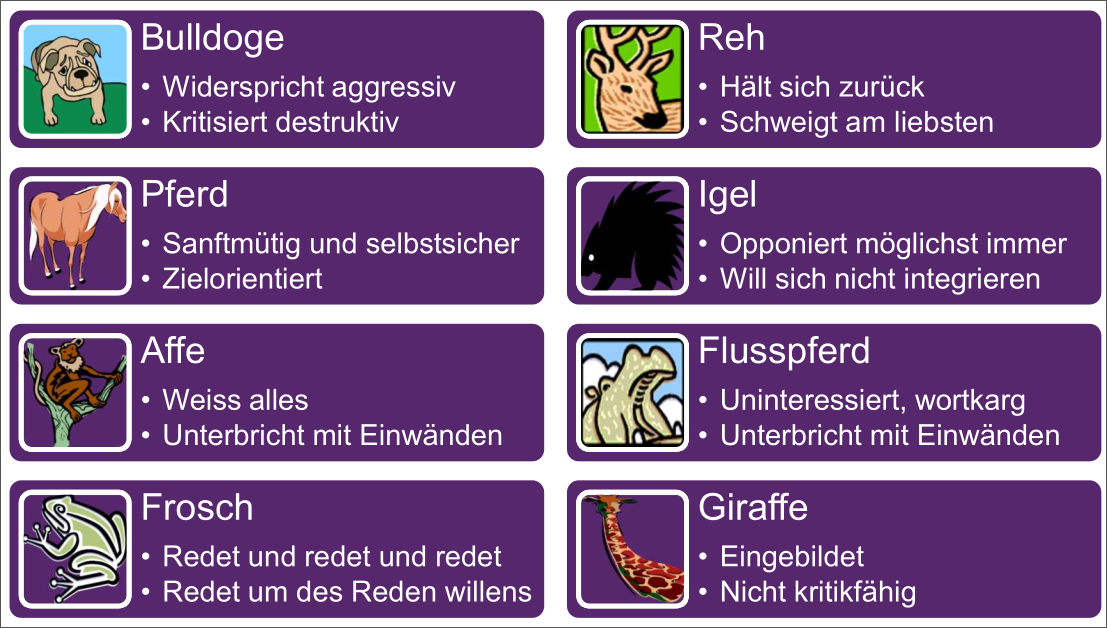
\includegraphics[scale=0.3]{2023_01_10_02_03_24.png}

\subsection{Negotiation Techniques}
\subsubsection{Harvard-Method}
\begin{enumerate}
\item \textcolor{purple}{Don't discuss what the discussion partner wants, but also why}
\item \textcolor{purple}{Try to understand the position of the discussion partner and help them understand your position as well}
\item \textcolor{purple}{try to act constructive to the discussion partners demands}
\item \textcolor{purple}{Try to find common ground}
\item \textcolor{purple}{Keep the negotiation alive, even when it seems that the negotiation failed}
\end{enumerate} 

\subsubsection{Compromise vs Consensus}
A compromise means that people will need to take a hit in their goals, a consensus means that you both found common ground where no one has to lose.\newline
Usually this means leaving a different part of the negotiation away and deal with that later, but implement the part that is beneficial for both parties, instead of trying to negotiate something that the other party clearly does not want.

\subsubsection{Conflict-Escalation (Friedrich Glas)}
\begin{itemize}
\item \textcolor{green}{WIN-WIN}\newline
  \begin{itemize}
  \item \textcolor{purple}{Increase in "roughness" (Verhärtung)}\newline
    conflict begins with "tension"
  \item \textcolor{purple}{Debate}\newline
    Difference in opinion, apply force to negotiation partner
  \item \textcolor{purple}{Action over words}\newline
    Empathy slowly gets lost, nonverbal
  \end{itemize} 
\item \textcolor{orange}{WIN-LOSE}
  \begin{itemize}
  \item \textcolor{purple}{Coalitions}\newline
    Attack/denounce the negotiation partner
  \item \textcolor{purple}{Lose of Face}\newline
    Ad-hominem attacks
  \item \textcolor{purple}{Threat strategies}\newline
    show of force
  \end{itemize} 
\item \textcolor{red}{LOSE-LOSE}
  \begin{itemize}
  \item \textcolor{purple}{Limited destruction}\newline
    cause damage to the opponent
  \item \textcolor{purple}{Destruction}\newline
    Destroy the system of the opponent
  \item \textcolor{purple}{mutually assured destruction}\newline
  \end{itemize} 
\end{itemize}

\subsubsection{Conflict (Virginia Satir)}
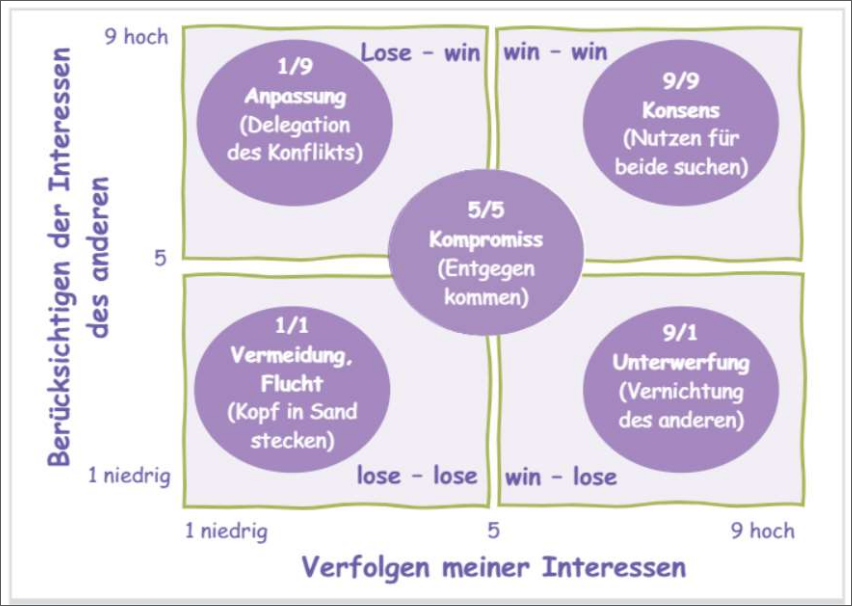
\includegraphics[scale=0.3]{2023_01_10_02_18_51.png}

\section{IT ServiceManagement}
\subsection{Business Usage}
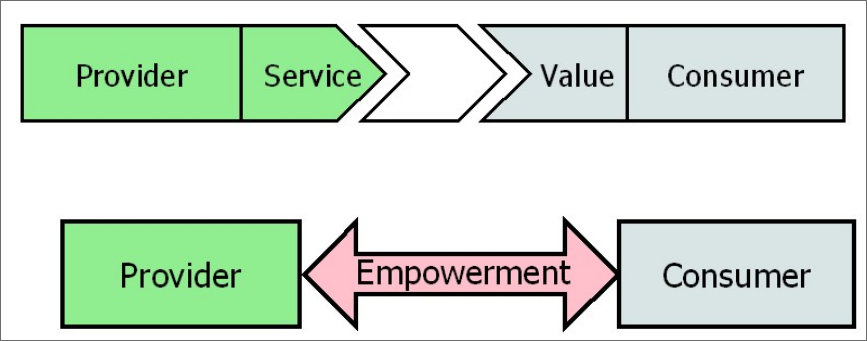
\includegraphics[scale=0.3]{2023_01_10_03_14_32.png}\newline
A customer would like the ROI to be 0 very fast, as the customer obviously wants to see returns from their investment. 

\subsection{Utility and Warranty}
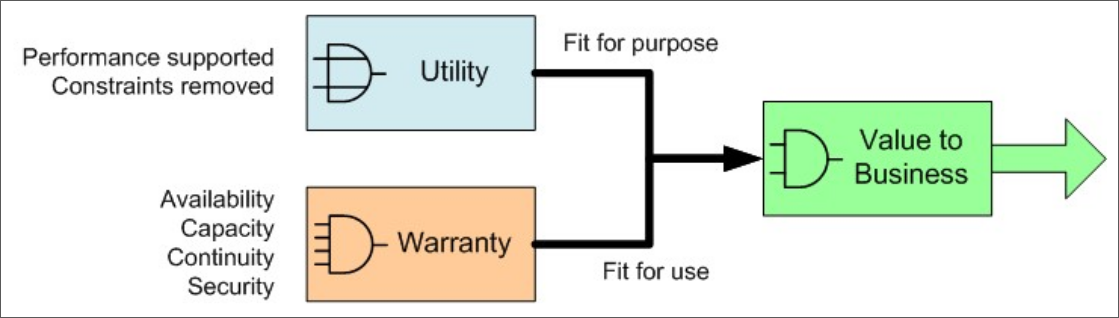
\includegraphics[scale=0.3]{2023_01_10_03_15_26.png}\newline
\textcolor{purple}{Utility -> Fit for purpose}\newline
\textcolor{purple}{Warranty -> Fit for use}\newline
Both the \textbf{utility and warranty need to be fulfilled in order for the product to be usable.} 

\subsection{Sections of Service Management}
\begin{itemize}
\item \textcolor{purple}{Organization}\newline
  \begin{itemize}
  \item \textcolor{black}{Structure}
  \item \textcolor{black}{Culture}
  \item \textcolor{black}{Capacity}
  \item \textcolor{black}{Skills}
  \item Management
  \item Communication
  \item Cooperation
  \end{itemize} 
\item \textcolor{purple}{Information}\newline
  \begin{itemize}
  \item \textcolor{black}{Technology}
  \item \textcolor{black}{Knowledge}
  \item \textcolor{black}{Inputs}
  \item \textcolor{black}{Outputs}
  \item Relationship
  \end{itemize} 
\item \textcolor{purple}{Partner \& Supplier}\newline
  \begin{itemize}
  \item \textcolor{black}{Relationship}
  \item \textcolor{black}{Contracts}
  \item \textcolor{black}{Agreements}
  \end{itemize} 
\item \textcolor{purple}{Value Streams}\newline
  \begin{itemize}
  \item \textcolor{black}{Processes}
  \item \textcolor{black}{Activities}
  \item \textcolor{black}{Workflows}
  \item \textcolor{black}{Controls}
  \item Procedures
  \end{itemize} 
\end{itemize} 

\subsection{Service Value System}
This is simply the process of turning the left side (ex. user story) into the wanted right side, (ex. completed user story).\newline
The middle here are the resources that are available to us.\newline
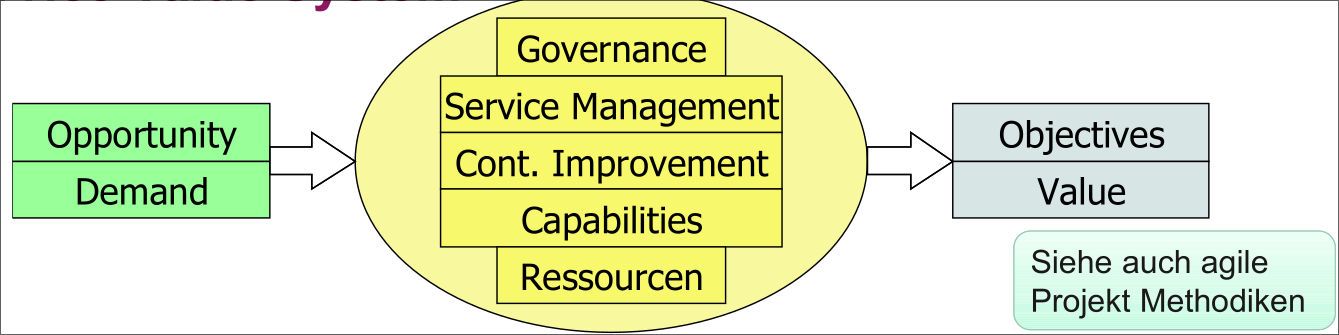
\includegraphics[scale=0.3]{2023_01_10_03_23_38.png}\newline
\textcolor{purple}{The problem here is that often there are echo chambers that will not properly work with each other, this is in general a problem for agile development, as agile only works if everyone works with everyone. Echo chambers can therefore ruin the entire process.}

\subsection{Resilience and Flexibility}
There is a fundamental difference between resilience and flexibility, namely the fact that flexibility is change for good, while resilience means being stand fest against change for the worse.\newline
Ex. in an economic crisis it might be a good thing to be resilient against layoffs, while being flexible with new technologies is in general a good thing. \newline
\textcolor{purple}{Another aspect is the influence from third parties, often these are not welcome and resilience to change caused by third party considered a good thing.}

\subsection{Principles of ITIL}
\begin{itemize}
\item \textcolor{purple}{Focus on usage}
\item \textcolor{purple}{Start at the current point, not at a theoretical one}
\item \textcolor{purple}{Do small steps and check these steps}
\item \textcolor{purple}{Cooperate and further transparency}
\item \textcolor{purple}{think and act at the same time (WAT LMAO)}
\item \textcolor{purple}{Keep it simple and practical}
\item \textcolor{purple}{optimize and automatize}
\end{itemize}
\textcolor{teal}{sounds like agile kekw}

\subsection{Service Value Chain}
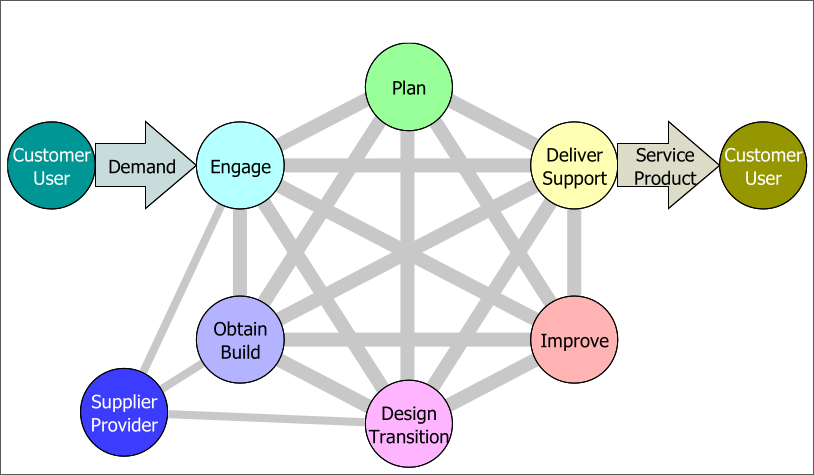
\includegraphics[scale=0.3]{2023_01_10_03_30_48.png}\newline
\begin{itemize}
\item \textcolor{purple}{Plan}\newline
  current status and direction
\item \textcolor{purple}{Improve}\newline
  continuous improvements on all activities in the value chain
\item \textcolor{purple}{Engage}\newline
  Understanding of requirements, transparency and engagement
\item \textcolor{purple}{Design \& Transition}\newline
  Quality, cost and time to market must be fulfilled
\item \textcolor{purple}{Obtain or Build}\newline
  Either buy or build the components at the right time and the right place
\item \textcolor{purple}{Deliver and Support}\newline
  deliver services and provide support
\end{itemize} 

\subsection{General Management Practices}
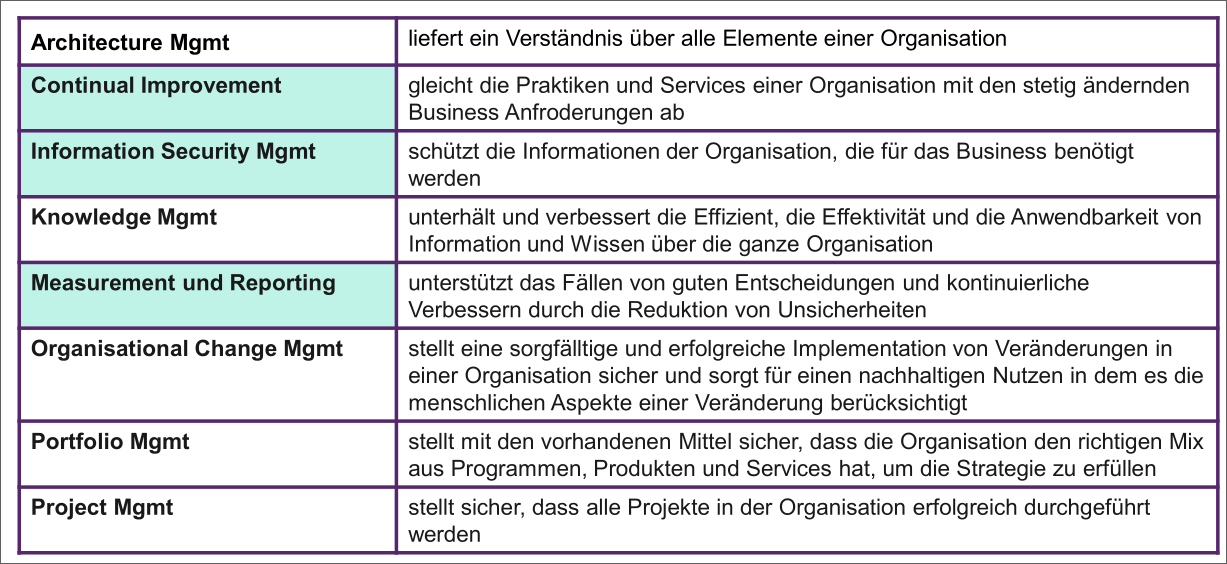
\includegraphics[scale=0.3]{2023_01_10_03_42_51.png}\newline
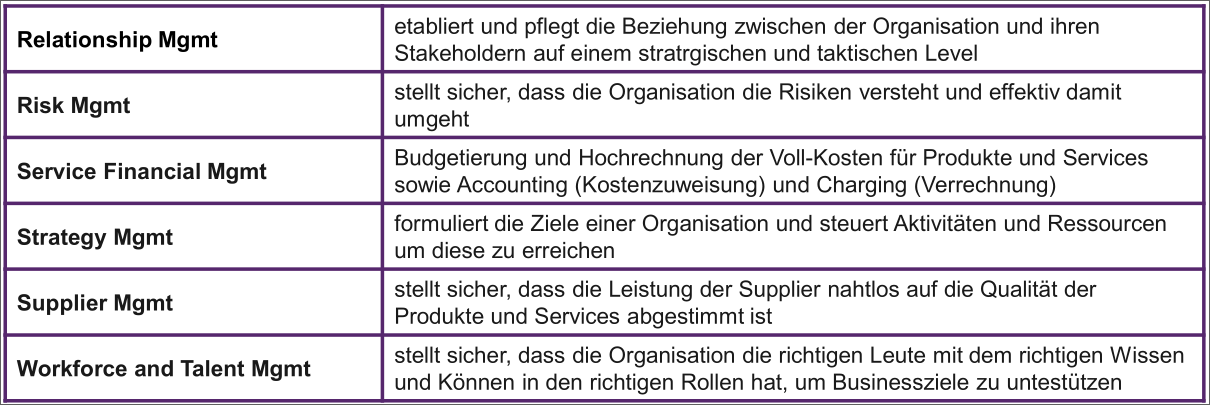
\includegraphics[scale=0.3]{2023_01_10_03_43_35.png}

\subsection{Service Management Practices}
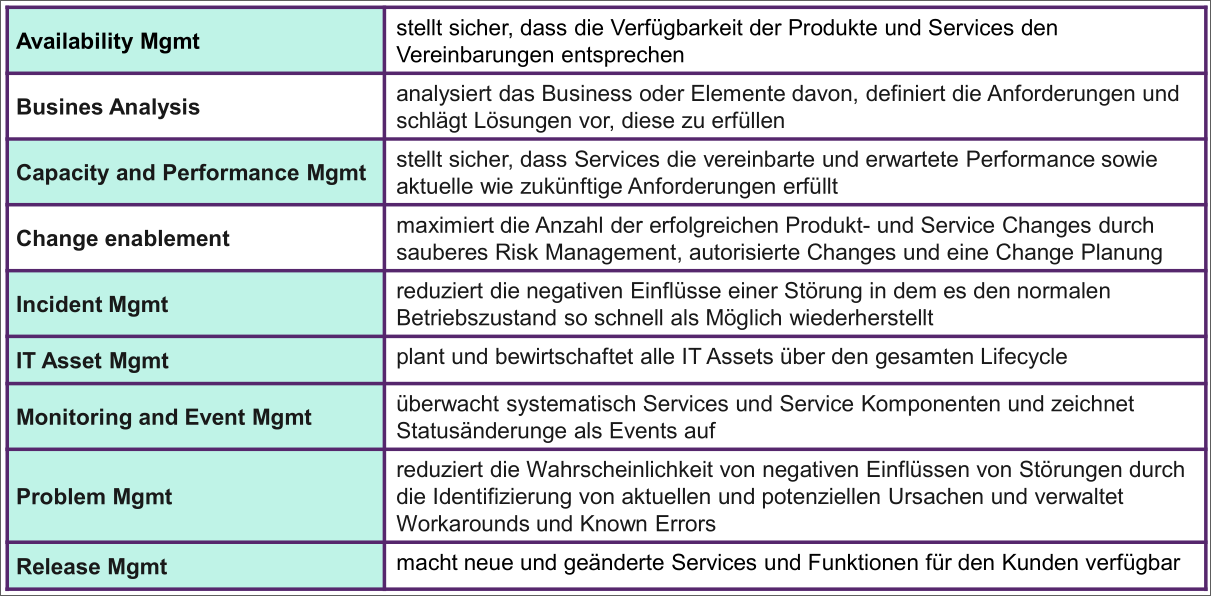
\includegraphics[scale=0.3]{2023_01_10_03_44_25.png}\newline
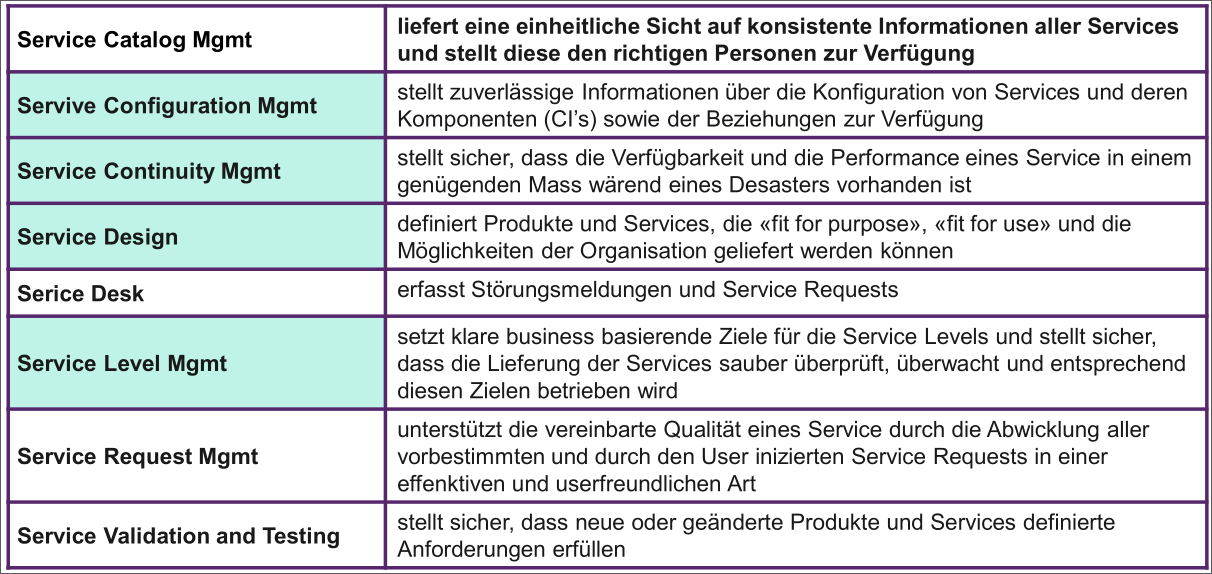
\includegraphics[scale=0.3]{2023_01_10_03_44_34.png}

\subsubsection{Service Design}
Deliver something new, while not breaking something that already exists and ensure that the service at the end will return the ROI for the customer.\newline
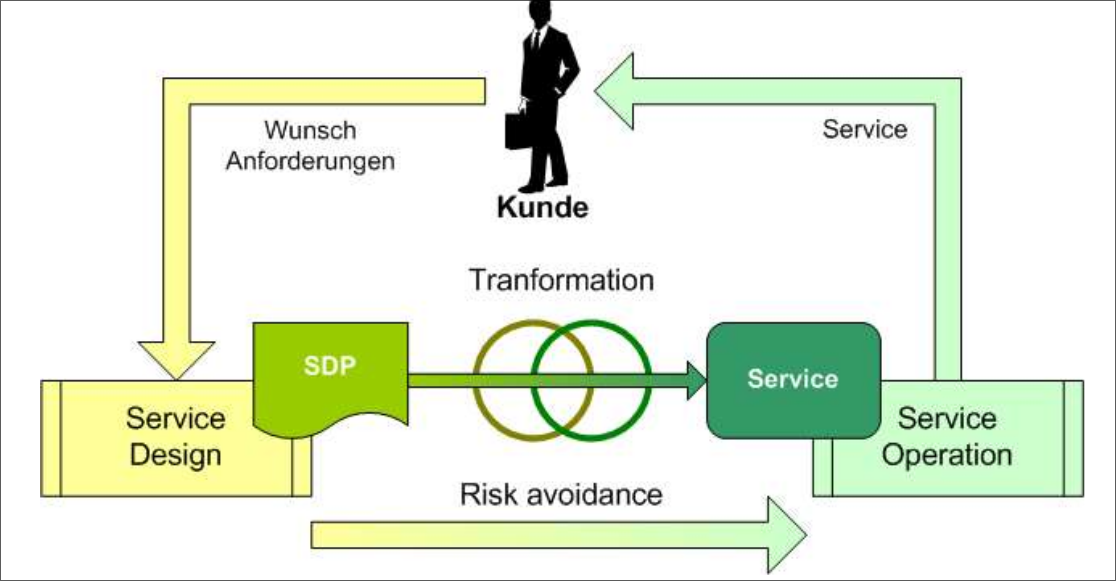
\includegraphics[scale=0.3]{2023_01_10_03_46_23.png}

\subsubsection{Service Level Management}
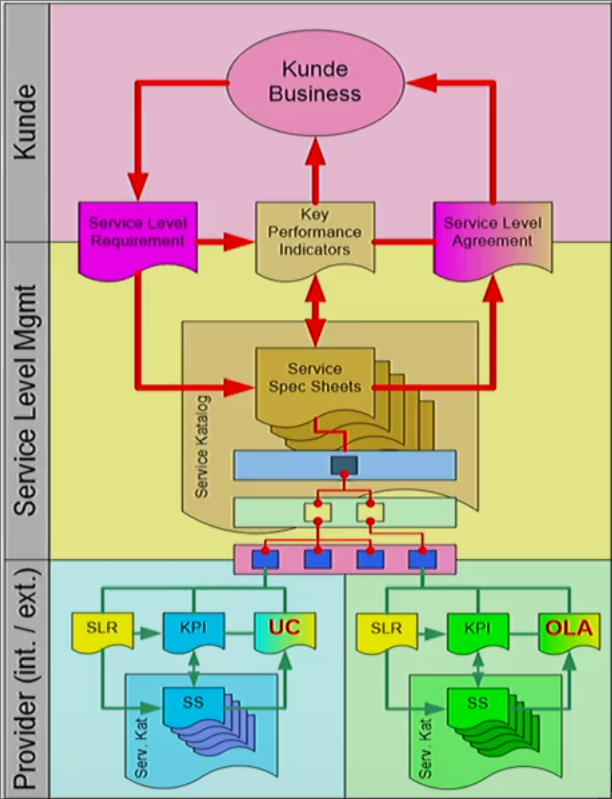
\includegraphics[scale=0.3]{2023_01_10_03_47_49.png}

\subsubsection{Capacity Management}
Ask the customer, what do you need \textbf{exactly?}\newline
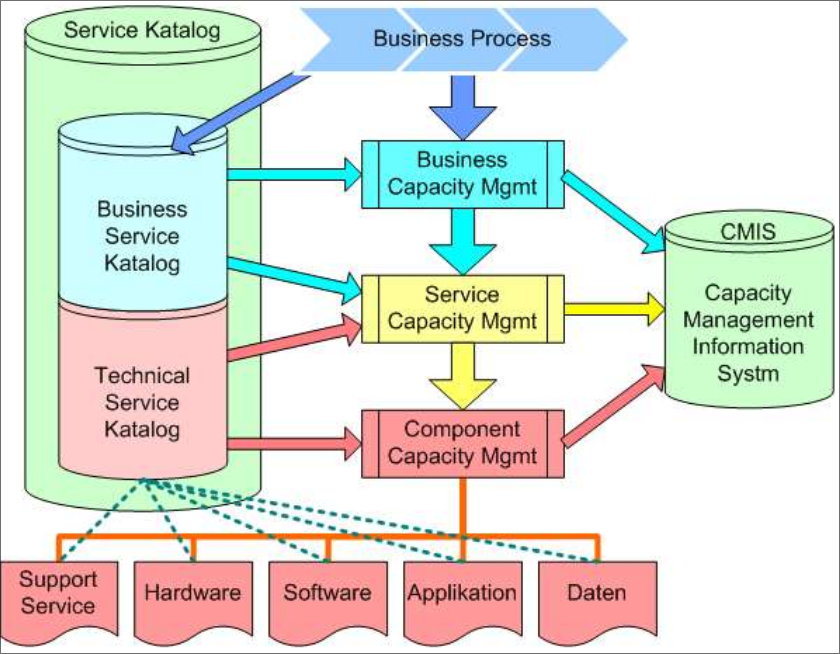
\includegraphics[scale=0.3]{2023_01_10_03_48_06.png}

\subsubsection{Availability Management}
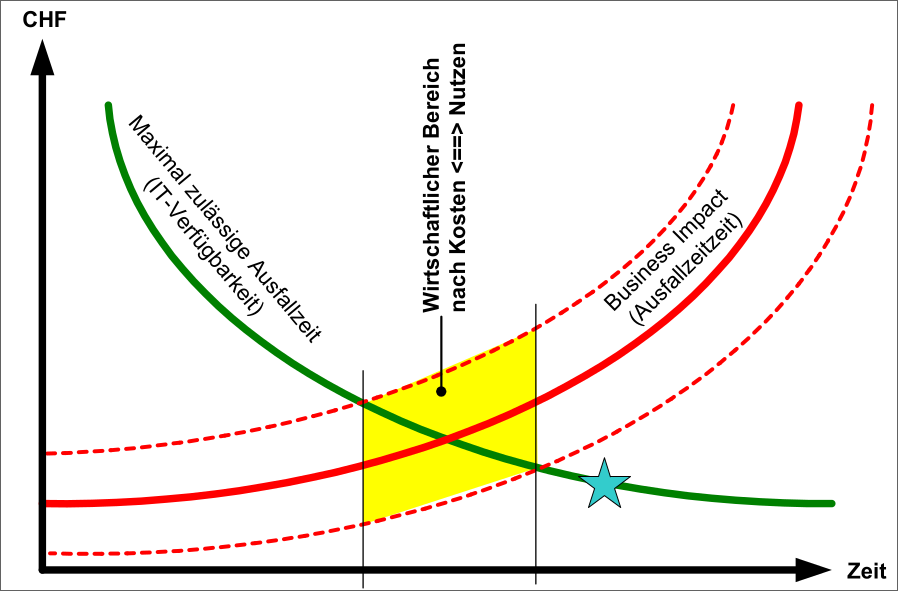
\includegraphics[scale=0.3]{2023_01_10_03_49_14.png}

\subsubsection{IT Asset and Service Configuration Management}
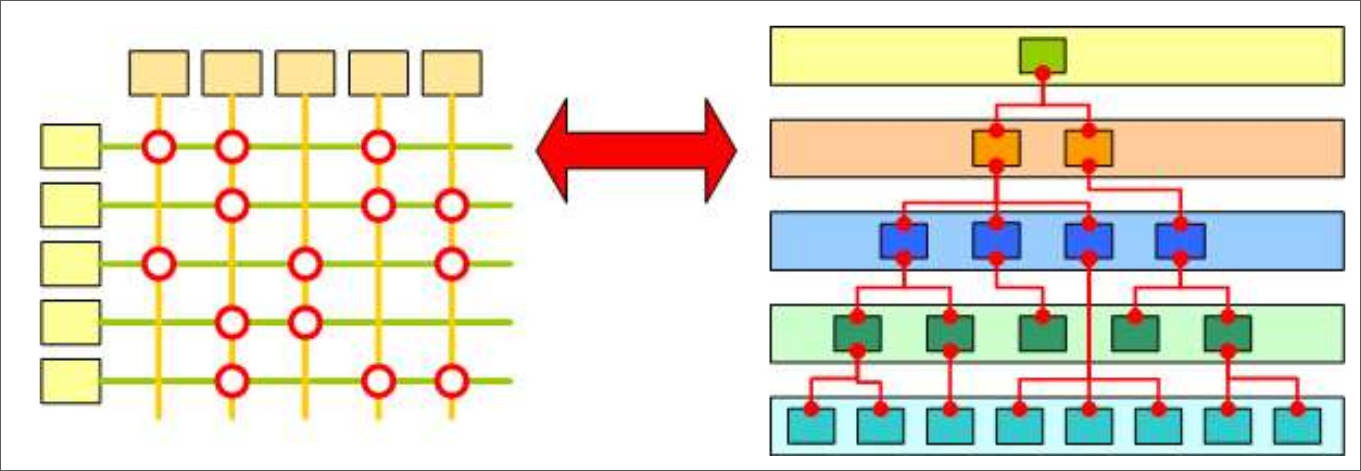
\includegraphics[scale=0.28]{2023_01_10_03_49_28.png}

\subsubsection{Service Desk and Incident Management}
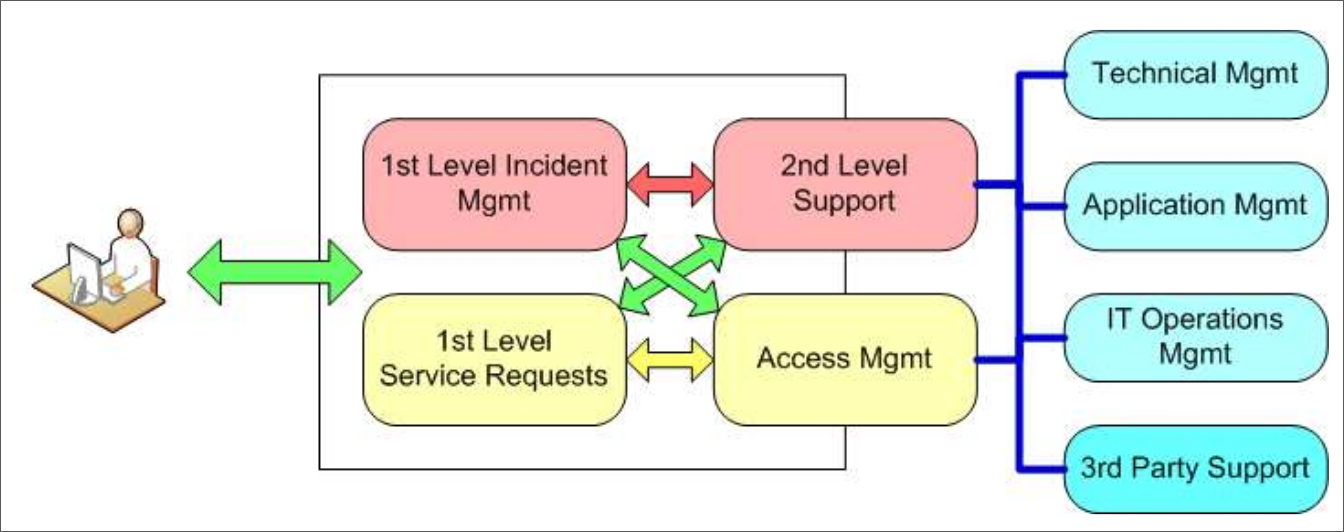
\includegraphics[scale=0.3]{2023_01_10_03_49_42.png}

\subsubsection{Problem Management}
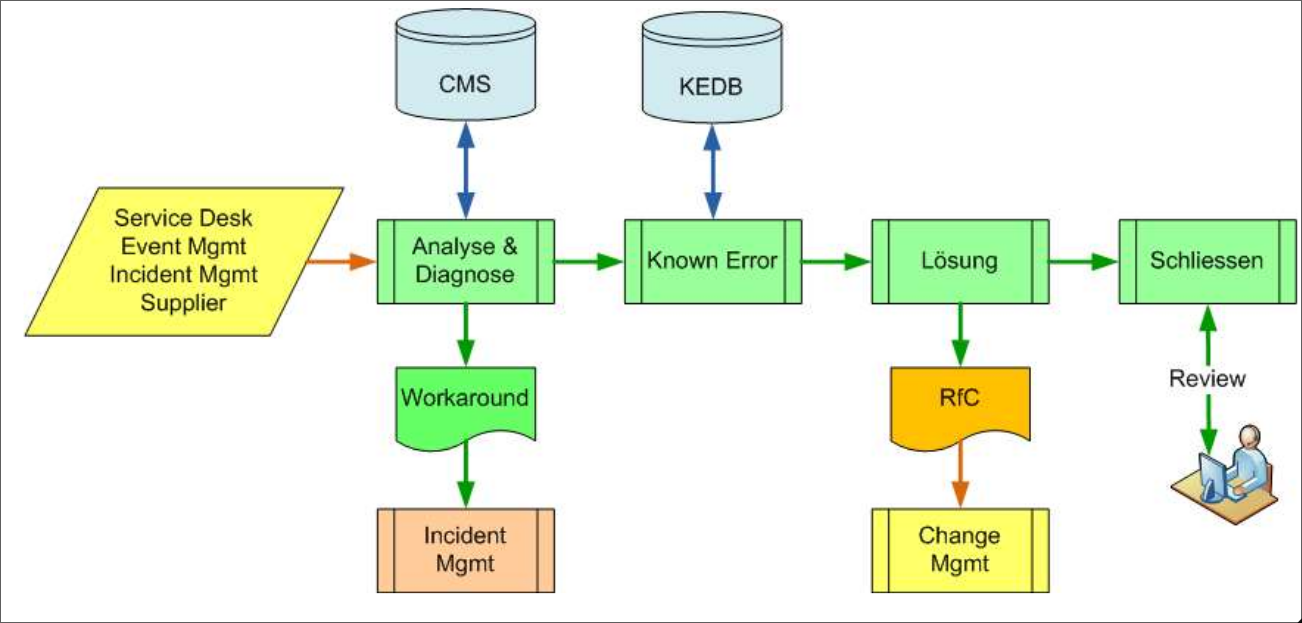
\includegraphics[scale=0.3]{2023_01_10_03_50_03.png}

\subsubsection{Incident - Problem - Change}
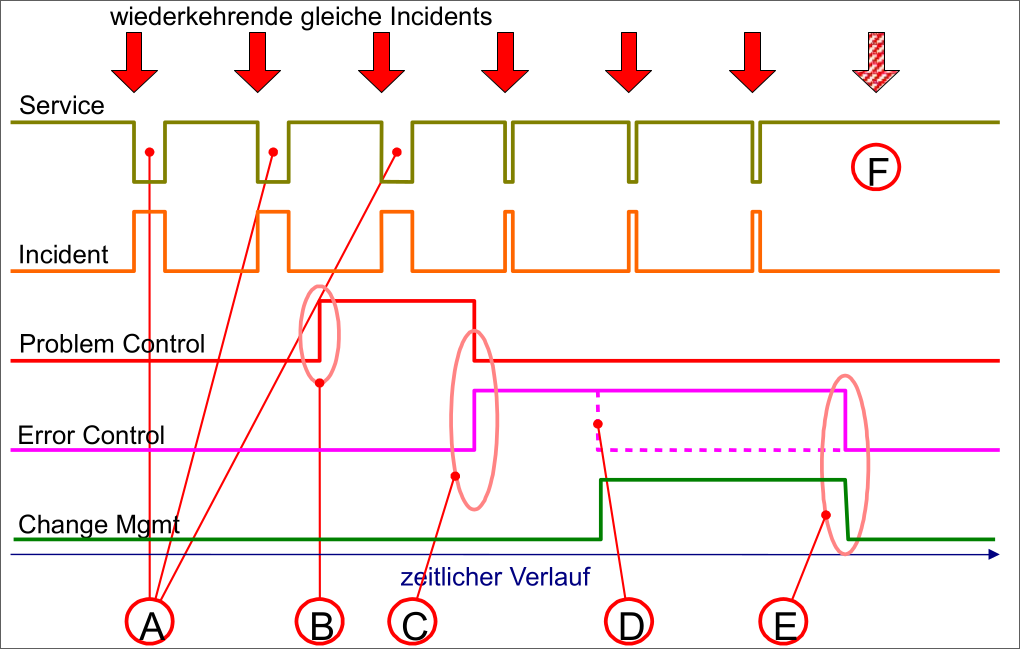
\includegraphics[scale=0.3]{2023_01_10_03_50_31.png}

\subsubsection{Monitoring and Event Management}
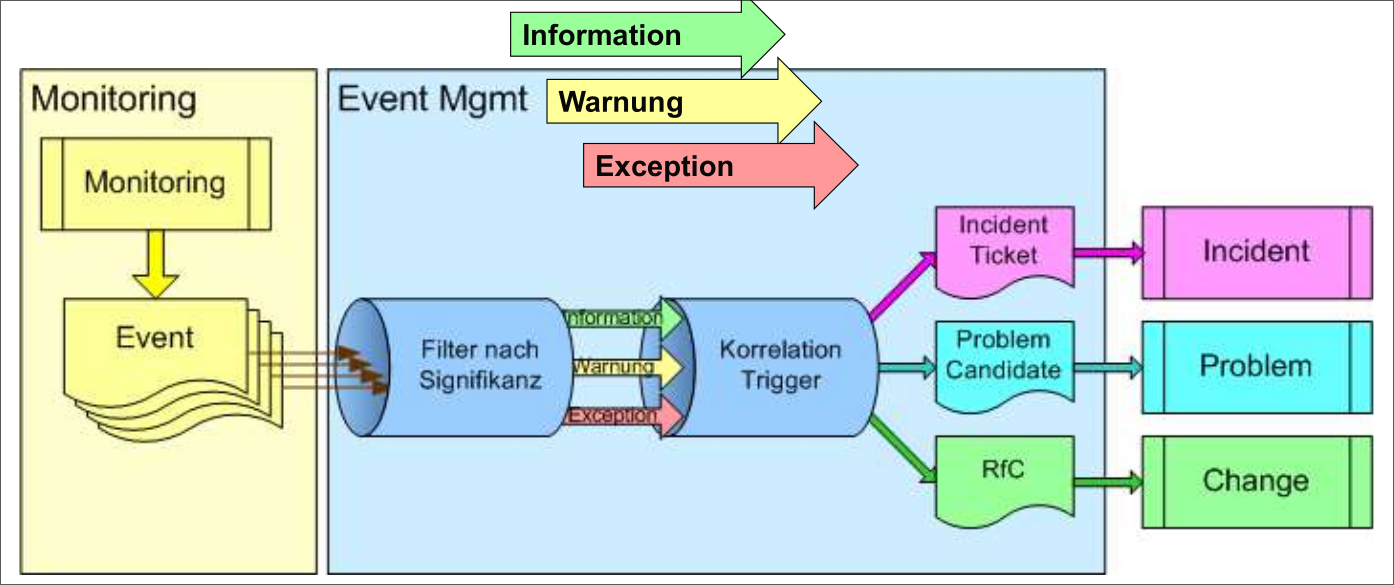
\includegraphics[scale=0.28]{2023_01_10_03_50_57.png}

\subsubsection{Service Continuity Management}
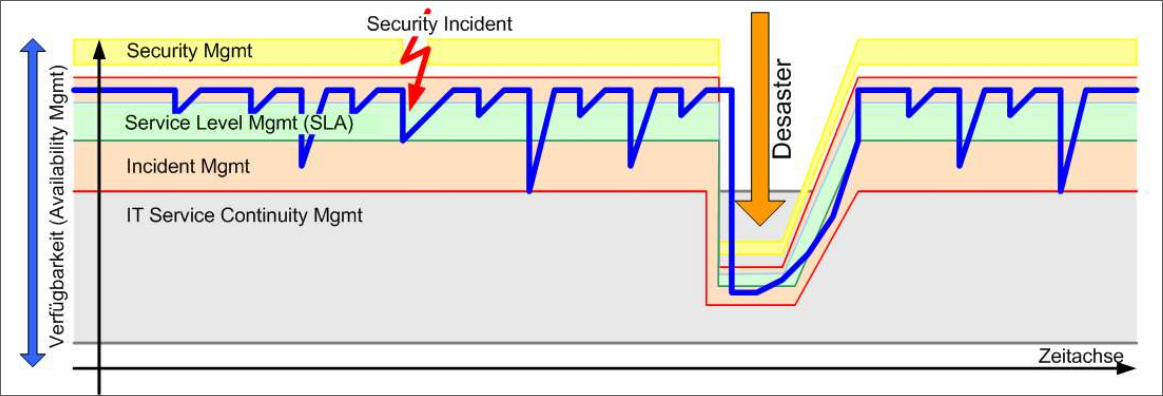
\includegraphics[scale=0.3]{2023_01_10_03_51_07.png}

\subsection{Technical Management Practises}
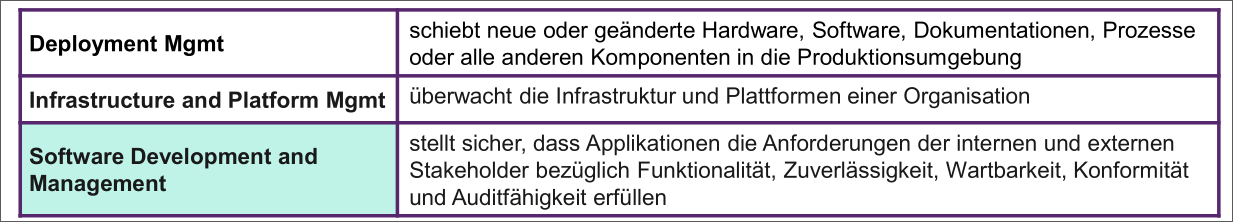
\includegraphics[scale=0.3]{2023_01_10_03_52_06.png}

\subsubsection{Change and Release Management (conventional)}
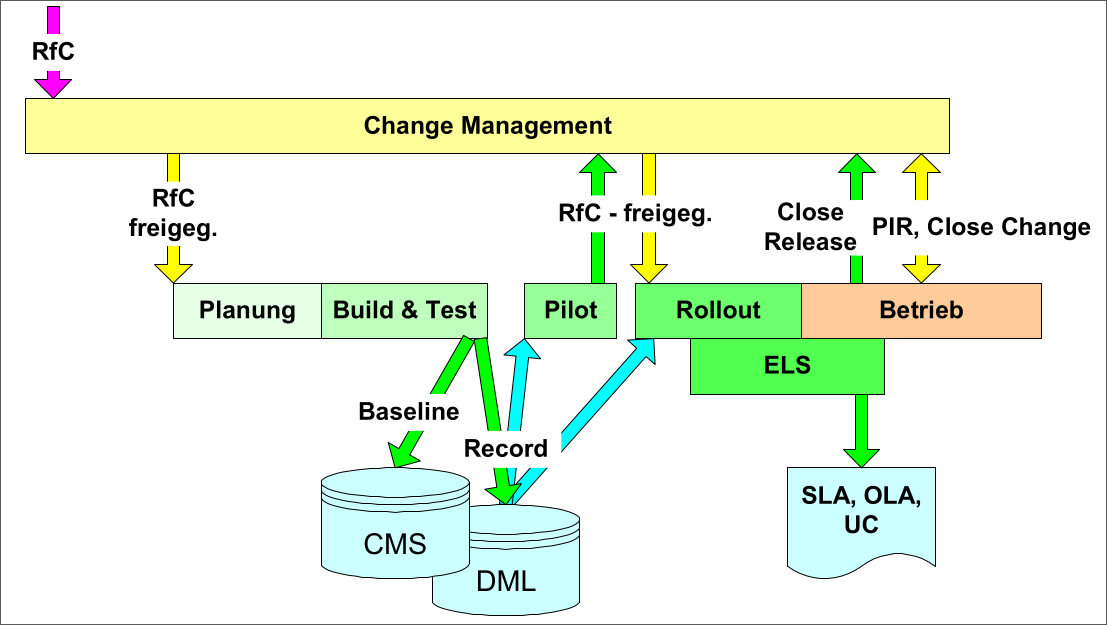
\includegraphics[scale=0.3]{2023_01_10_03_52_14.png}

\subsubsection{Change and Release Management (agile)}
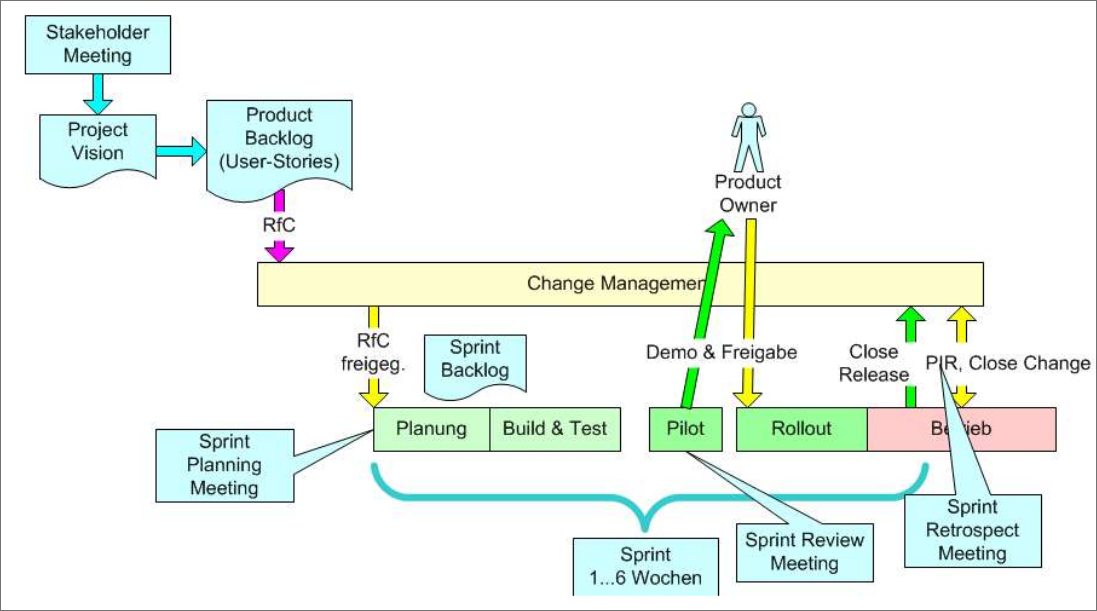
\includegraphics[scale=0.3]{2023_01_10_03_52_44.png}

\subsection{Infrastructure and Platform Management}
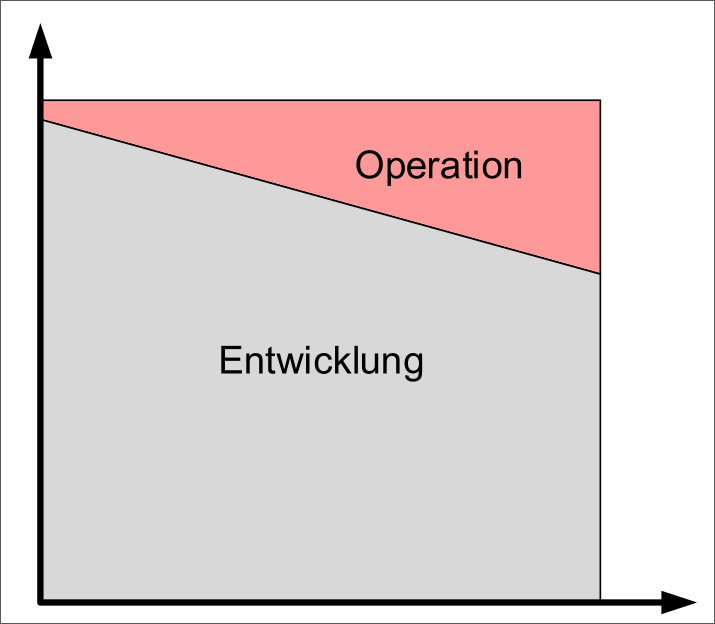
\includegraphics[scale=0.3]{2023_01_10_03_53_34.png}\newline
\textcolor{purple}{Dev-Ops teams need up to 30\% of the resources for their operation!}


\end{multicols*}
\end{document}
